\title{Extrapolating expected accuracies for multi-class classification}
\author{Charles Zheng, Rakesh Achanta and Yuval Benjamini}
\date{\today}

\documentclass[12pt]{article} 

% packages with special commands
\usepackage{amssymb, amsmath}
\usepackage{epsfig}
\usepackage{array}
\usepackage{ifthen}
\usepackage{color}
\usepackage{fancyhdr}
\usepackage{graphicx}
\usepackage{mathtools}
\usepackage{csquotes}
\usepackage{multirow}
\usepackage{xcolor}
\usepackage{chngcntr}
\usepackage{apptools}
\AtAppendix{\counterwithin{lemma}{section}}
\usepackage[backend=bibtex,style=authoryear]{biblatex}


\addbibresource{example.bib} % The filename of the bibliography

\newcommand\crule[3][black]{\textcolor{#1}{\rule{#2}{#3}}}

\definecolor{grey}{rgb}{0.5,0.5,0.5}
\definecolor{color1}{RGB}{128,13,13}
\definecolor{color2}{RGB}{70,128,13}
\definecolor{color3}{RGB}{13,128,128}
\definecolor{color4}{RGB}{70,13,128}

\begin{document}
\maketitle

\newcommand{\skone}{\mathcal{S}_{k_1}}
\newcommand{\sktwo}{\mathcal{S}_{k_2}}

\newcommand{\tr}{\text{tr}}
\newcommand{\E}{\textbf{E}}
\newcommand{\diag}{\text{diag}}
\newcommand{\argmax}{\text{argmax}}
\newcommand{\Cov}{\text{Cov}}
\newcommand{\Var}{\text{Var}}
\newcommand{\argmin}{\text{argmin}}
\newcommand{\Vol}{\text{Vol}}
\newcommand{\comm}[1]{}
\newcommand{\indep}{\rotatebox[origin=c]{90}{$\models$}}
\newcommand{\Cor}{\text{Cor}}
\newtheorem{theorem}{Theorem}[section]
\newtheorem{proposition}{Proposition}[section]
\newtheorem{corollary}{Corollary}[theorem]
\newtheorem{lemma}{Lemma}[section]
\newtheorem{definition}{Definition}[section]
\newcommand{\bZ}{\boldsymbol{Z}}
\newcommand{\bz}{\boldsymbol{z}}
\newcommand{\bx}{\boldsymbol{x}}
\newcommand{\bX}{\boldsymbol{X}}

\newcommand{\bH}{\boldsymbol{H}}


\begin{abstract}
The difficulty of multi-class classification generally increases with
the number of classes.  Using data from a subset of the classes, can
we predict how well a classifier will scale with an increased number
of classes?  Under the assumption that the classes are sampled
exchangeably, and under the assumption that the classifier is
generative (e.g. QDA or Naive Bayes), we show that the expected
accuracy when the classifier is trained on $k$ classes is the $k-1$st
moment of a \emph{conditional accuracy distribution}, which can be
estimated from data.  This provides the theoretical foundation for
performance extrapolation based on pseudolikelihood, unbiased
estimation, and high-dimensional asymptotics.  We investigate the
robustness of our methods to non-generative classifiers in simulations
and one optical character recognition example.
\end{abstract}

As we foreshadowed in the introduction, randomized classification is
also one of the three methods we consider for evaluating
representations.  Yet, two other applications of randomized
classification are (i) for providing a formalism for evaluting
\emph{recognition systems}, and (ii) for studying generalizability of
certain classification-based experiments.  The application of
recognition systems provides the most intuitive way of understanding
the randomized classification task; therefore, in this chapter, we
begin with a discussion in section \ref{sec:recog_tasks} of
recognition tasks, and within this context, motivate the definition of
a randomized classification task in section \ref{sec:rc_motivation}.
We propose to use the randomized classification task to model the
problem of recognition, and to evalaute performance via the
\emph{average accuracy}.  Next, to put our ideas into practice, we
need ways to estimate the average accuracy from data, which we address
in \ref{sec:estimation_average_accuracy}.


\section{Recognition tasks}\label{sec:recog_tasks}

Human brains have a remarkable ability to recognize objects, faces,
spoken syllables and words, and written symbols or words, and this
recognition ability is essential for everyday life.  While researchers
in artificial intelligence have attempted to meet human benchmarks for
these classical recognition tasks for the last few decades, only very
recent advances in machine learning, such as deep neural networks,
have allowed algorithmic recognition algorithms to approach or exceed
human performance (\cite{lecun2015deep}).

Within the statistics and machine learning literature, the usual
formalism for studying a recognition task is to pose it as a
\emph{multi-class classification} problem.  One delineates a finite
set of distinct entities which are to be recognized and distinguished,
which is the \emph{label set} $\mathcal{Y}$.  The input data is
assumed to take the form of a finite-dimensional real \emph{feature
  vector} $X \in \mathbb{R}^p$.  Each input instance is associated
with exactly one true label $Y \in \mathcal{Y}$.  The solution to the
classification problem takes the form of an algorithmically
implemented \emph{classification rule} $h$ that maps vectors $X$ to
predicted labels $\hat{Y} \in \mathcal{Y}$.  The classification rule
can be constructed in a data-dependent way: that is, one collects a
number of labelled \emph{training observations} $(X_1, Y_1)$ which is
used to inform the construction of the classification rule $h$.  The
quality of the classification rule $h$ is measured by \emph{generalization accuracy}
\[
\text{GA}(h) = \Pr[h(X) = Y],
\]
where the probability is defined with reference to the unknown
population joint distribution of $(X, Y)$.  

However, a limitation of the usual multi-class classification
framework for studying recognition problems is the assumption that the
label set $\mathcal{Y}$ is finite and known in advance.  When
considering human recognition capabilities, it is clear that this is
not the case.  Our ability to recognize faces is not limited to some
pre-defined, fixed set of faces; same with our ability to recognize
objects in the environment.  Humans learn to recognize novel faces and
objects on a daily basis.  And, if artificial intelligence is to fully
match the human capability for recognition, it must also possess the
ability to add new categories of entities to its label set over time;
however, at present, there currently exists a void in the machine
learning literature on the subject of the online learning of new
classes in the data.

The central theme of this thesis is the study of \emph{randomized
  classification}, which can be motivated as an extension of the
classical multi-class classification framework to accommodate the
possibility of growing or infinite label sets $\mathcal{Y}$. The basic
approach taken is to assume an infinite or even continuous label space
$\mathcal{Y}$, and then to study the problem of classification on
finite label sets $S$ which are randomly sampled from $\mathcal{Y}.$
This, therefore defines a \emph{randomized classification} problem
where the label set is finite but may vary from instance to instance.
One can then proceed to answer questions about the variability of the
performance due to randomness in the labels, or how performance
changes depending on the size of the random label set.

\section{Randomized classification}\label{sec:rc_motivation}

\subsection{Motivation}
The formalism of classification is inadequate for studying many
practical questions related to the generalizability of the facial
recognition system.  Using test data, we estimate the generalization
accuracy of a recognition system.  However, these estimated accuracies
apply only to the particular collection of individuals
$\{y^{(1)},\hdots, y^{(k)}\}$.  If we were to add a new individual
$y^{(k+1)}$ to the dataset, for instance, when photographs are
uploaded on Facebook containing a new user, this defines a totally new
classification problem because the expanded set of labels
$\{y^{(1)},\hdots, y^{(k+1)}\}$ defines a different response space
than the old set of labels $\{y^{(1)},\hdots, y^{(k)}\}$.  Yet, these
two classification problems are clearly linked.  To take another
example, a client might want to run a facial recognition system
developed by lab A on their own database of individuals.  In this
case, there might be no overlap between the people in lab A's database
and the people in the client's database.  And yet, the client might
still expect the performance figures reported by lab A to be
informative of how well the recognition system will do on their own
database!

The question of how to link performance between two different but
related classification tasks is an active area of research, known as
\emph{transfer learning}.  But while the two examples we just listed
might be considered as examples of transfer learning problems, the
current literature on transfer learning, as far as we know, does not
study the problem of \emph{mutating label sets}.  Therefore, to
address this new class of questions about the generalizability of the
recognition system, we need to formalize our notions of (a) what
constitutes a `recognition system' which can be applied to different
classification problems, and (b) what assumptions about the problem,
and what assumptions about the classifiers used, allow one to infer
performance in one classification problem based on performance in
another classification problem.

\subsection{Setup}
By `recognition system,' we really mean a \emph{learning algorithm}
$\Lambda$ which can take training data as input, and produce a
classification rule for recognizing faces.  While a classification
rule is bound to a specific label set, a learning algorithm can be
applied to datasets with arbitrary label sets, and be continually
updated as new labels are added to the label set.  To `update' a
facial recognition system with new data means to apply the learning
algorithm to the updated database.

Now we can formalize what it means to generalize performance from one
problem to another.  A \emph{classification problem} $P$ is specified
by a label set $\mathcal{Y}$, a predictor space $\mathcal{X}$, a joint
distribution $G$ on $\mathcal{X} \times \mathcal{Y}$, and a
\emph{sampling scheme} $S$ for obtaining training data (for example,
to obtain $n$ observations from $G$ i.i.d.).  The sampling scheme is
needed because we cannot say much about how the learning algorithm
will perform unless we know how much training data it is going to
have.  The generalization accuracy (GA) of the algorithm $\Lambda$ on the
classification problem $P = (\mathcal{Y}, \mathcal{X}, G, S)$ is
defined as the expected risk of the resulting classification rule $h$,
\[
\text{GA}_P(\Lambda) = \E[\text{GA}(h)]
\]
where $h$ is produced by applying $\Lambda$ to the training data,
sampled by $S$.  The expectation is taken over the randomness in the
generation of the training data.

At this point we have defined an extremely general transfer learning
problem: given two different classification problems $P_1 =
(\mathcal{Y}_1, \mathcal{X}_1, G_1, S_1)$ and $P_2 = (\mathcal{Y}_2,
\mathcal{X}_2, G_2, S_2)$, what can we say about the relationship
between $\text{GA}_{P_1}(\Lambda)$ and $\text{GA}_{P_2}(\Lambda)$?
Not much, unless we make many more assumptions about how $P_1$ and
$P_2$ are linked.

The basic approach we will take is to assume that both $P_1$ and $P_2$
have been generated randomly via a common mechanism.  In the original
motivating context of facial recognition, this is to say that two
different label sets $\mathcal{Y}_1$ and $\mathcal{Y}_2$ are linked
because they both belong to a common population of labels
$\mathcal{Y}$, i.e., the population of all possible humans, and to
further assume that both have been \emph{sampled}, in the same manner,
from $\mathcal{Y}$.

The study of how to make inferences about the risk in $P_2$ given
information about the performance achieved in $P_1$, granted a set of
assumptions on how $P_1$ and $P_2$ have been randomly generated (and
are thereby linked through shared randomization mechanisms) forms the
basis of the subject of \emph{randomized classification}.

As we noted in the introduction, the problem of randomized
classification has a close ancestor in the study of \emph{random code
  models} in information theory.  There, the problem is to understand
the \emph{decoding performance} (the analogue to risk) of a
encoding/decoding system $P$ which has a randomized code space
$\mathcal{Y}$.  Where random code models have a random codebook which
is a sample over a distribution of all possible codes, randomized
classification problems have a random label set that is a sample of a
larger label space.  However, the results we obtain for randomized
classification are more general in nature than the existing results
availible for random code models, because work on random codes is
generally limited to asymptotic settings, whereas we obtain finite-$k$
results, and because random code models assume a specific
product-distribution structure on $(X, Y)$ which is not appropriate
for classification problems.

\subsection{Assumptions}

The randomized classification model we study has the following
features.  We assume that there exists an infinite (or even
continuous) label space $\mathcal{Y}$ and a response space
$\mathcal{X} \in \mathbb{R}^p$.  For each label $y \in \mathcal{Y}$,
there exists a distribution of features $F_y$.  That is to say, that
for a feature-label pair $(X, Y)$, that the conditional distribution
of $X$ given $Y = y$ is given by $F_y$.  Furthermore, we assume that
there exists a prior distribution $\pi$ on the label space $\mathcal{Y}$.

A random classification task $P$ can be generated as follows.  The
label set $\mathcal{S} = \{Y^{(1)},\hdots, Y^{(k)}\}$ is generated by
drawing labels $Y^{(1)},\hdots, Y^{(k)}$ i.i.d. from $\pi$.  The joint
distribution $G$ of pairs $(X, Y)$ is uniquely specified by the two
conditions that (i) the marginal distribution of $Y$ is uniform over
$\mathcal{S}$, and (ii) the conditional distribution of $X$ given
$Y=Y^{(i)}$ is $F_{Y^{(i)}}$.  We sample both a training set and a
test set.  The training set is obtained by sampling $r_1$ observations
$X_{j, train}^{(i)}$ i.i.d. from $F_{Y^{(i)}}$ for $j = 1,\hdots,
r_1$.  The test set is likewise obtained by sampling $r_2$
observations $X_j^{(i)}$ i.i.d. from $F_{Y^{(i)}}$ for $j = 1,\hdots,
r_2$.  For notational convenience, we represent the training set as
the set of empirical distributions $\{\hat{F}_{Y^{(i)}}\}_{i=1}^k$
where
\[
\hat{F}_{Y^{(i)}} = \frac{1}{r_1} \sum_{j=1}^{r_1} \delta_{X^{(i)}_{j, train}}.
\]
Figure \ref{fig:training_set} illustrates the sampling scheme for
generating the training set.

\begin{figure}[h]
\centering
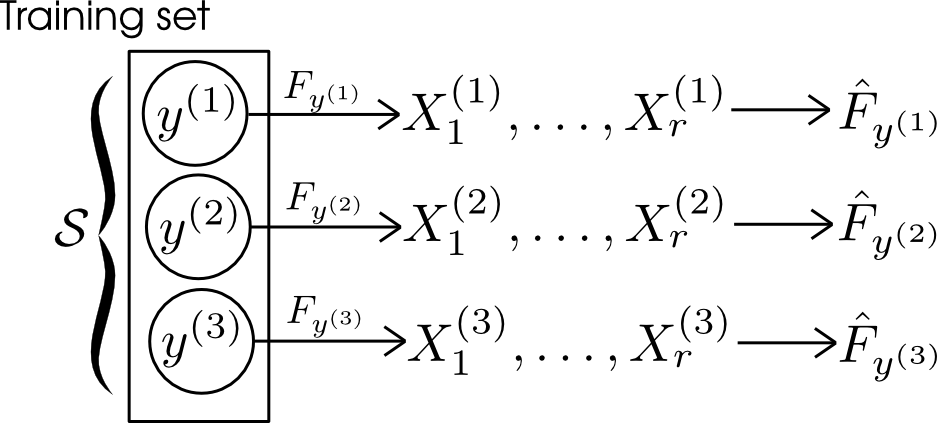
\includegraphics[scale = 0.4]{training_set.png}
\caption{Training set}\label{fig:training_set}
\end{figure}

Our analysis will also rely on a property of the classifier. We do not
want the classifier to rely too strongly on complicated interactions
between the labels in the set. We therefore propose the following
property of marginal separability for classification models:

\begin{definition}
\begin{enumerate}
\item The classification rule $h$ is called a \emph{marginal rule} if 
\[
h(x) = \text{argmax}_{y \in \mathcal{S}} m_y(x),
\]
where the function $m_y$ maps $\mathcal{X}$ to $\mathbb{R}$. 
\item Define a marginal model $\mathcal{M}$ as a mapping from empirical distributions
to margin functions,
\[
\mathcal{M}(\hat{F}_y) = m_y(x).
\]
\item A classifier that produces marginal classification rules
\[
h(x) = \text{argmax}_{y \in \mathcal{S}} m_y(x),
\]
by use of a marginal model, i.e. such that
$m_y=\mathcal{M}(\hat{F}_y)$ for some marginal model $\mathcal{M}$,
is called a \emph{marginal classifier}.
\end{enumerate}
\end{definition}
In words, a marginal classification rule produces a \emph{margin}, or
score, for each label, and chooses the label with the highest
margin. The marginal model converts empirical distributions
$\hat{F_y}$ over $\mathcal{X}$ into the margin function
$m_y$.  The \emph{marginal} property allows us to prove strong results
about the accuracy of the classifier under i.i.d. sampling assumptions.

\textbf{Comments:}
\begin{enumerate}
\item The marginal model includes several popular classifiers.
A primary example for a marginal model is the estimated Bayes
classifier. Let $\hat{f_y}$ be a density estimate obtained from the
empirical distribution $\hat{F_y}$. Then, we can use the estimated
densities of each class to produce the margin functions:
\[ m^{EB}_y(x) = \log(\hat{f_{y}}(x)).\]
The resulting empirical approximation for the Bayes classifier
(further assuming a uniform prior $\pi$) would be
\[ f^{EB}(x) = \text{argmax}_{y \in \mathcal{S}}(m^{EB}_y(x)).\]
\item Both the Quadratic Discriminant Analysis and the naive Bayes classifiers can be seen as specific instances of an estimated Bayes classifier
\footnote{QDA is the special case of the estimated Bayes classifier when $\hat{f_y}$ is obtained as
the multivariate Gaussian density with mean and covariance parameters estimated from the data.
Naive Bayes is the estimated Bayes classifier when $\hat{f_y}$ is obtained as the product of estimated componentwise marginal distributions
of $p(x_i|y)$}. 
For QDA, the margin function is
given by
\[
m_y^{QDA}(x) = -(x - \mu(\hat{F}_y))^T \Sigma(\hat{F}_y)^{-1} (x-\mu(\hat{F}_y)) - \log\det(\Sigma(\hat{F}_y)),
\]
where $\mu(F) = \int y dF(y)$ and $\Sigma(F) = \int (y-\mu(F))(y-\mu(F))^T dF(y)$.
In Naive Bayes, the margin function is
\[
m^{NB}_y(x) = \sum_{i=1}^n \log \hat{f}_{y, i}(x),
\]
where $\hat{f}_{y, i}$ is a density estimate for the $i$-th component of
$\hat{F}_y$.
\item There are also many classifiers which do not satisfy the marginal property, such as multinomial logistic regression,
multilayer neural networks, decision trees, and k-nearest neighbors.
\end{enumerate}

The operation of a marginal classifier is illustrated in figure
\ref{fig:classification_rule}.  Since a marginal classifier is
specified entirely by its marginal model $\mathcal{M}$, we will take
the notational convention of referring to a marginal classifier as
$\mathcal{M}$.

\begin{figure}[h]
\centering
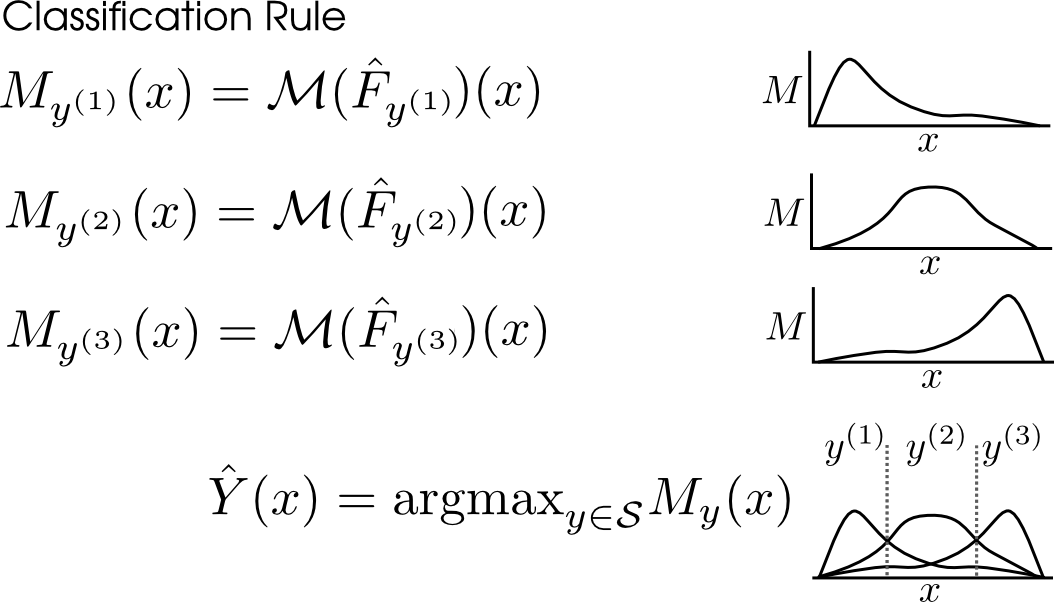
\includegraphics[scale = 0.4]{classification_rule.png}
\caption{Classification rule}\label{fig:classification_rule}
\end{figure}

We would like to identify the sources of randomness in evaluating a
classifier.  First, there is the specific choice of $k$ classes for
the label set.   Second, there is randomness in training the classifier
for these classes, which comes from the use of a finite training
set. Third, there is the randomness in the estimated risk when
testing the classifier on a test set.

If we \emph{fix} a particular realization of the random label set
$\mathcal{S} = \{y^{(1)}, \hdots, y^{(k)}\}$ as well as the training
set $\{\hat{F}_{y^{(i)}}\}_{i=1}^k$, then the classifier $h(x)$ is
fixed, and only the third source of randomness (in test risk) applies.
However, the true generalization accuracy of the classifier is deterministic:
\begin{align*}
\text{GA}(h) &= \Pr[Y = h(X)|Y \sim \text{Unif}(\mathcal{S}),
  \mathcal{S}, \{\hat{F}_{y^{(i)}}\}_{i=1}^k] 
\\&= \frac{1}{k}
\sum_{i=1}^k \Pr[m_{y^{(i)}}(x) = \max_j m_{y^{(j)}}(x)|X \sim
  F_{y^{(i)}}, \mathcal{S}, \{\hat{F}_{y^{(i)}}\}_{i=1}^k].  
\\&= \frac{1}{k}
\sum_{i=1}^k \int_{\mathcal{X}} I(m_{y^{(i)}}(x) = \max_j m_{y^{(j)}}(x)) dF_{y^{(i)}}(x),
\end{align*}
recalling that $m_{y^{(i)}}(x) \stackrel{def}{=}
\mathcal{M}(\hat{F}_{y^{(i)}})(x)$ is the margin function obtained
from the training data of the $i$th class.

If we \emph{fix} a particular realization of the random label set
$\mathcal{S} = \{y^{(1)}, \hdots, y^{(k)}\}$, then we can define the
(generalization) accuracy specific to that label set.  However, the
training data $\{\hat{F}_{y^{(i)}}\}_{i=1}^k$ will be random.  Let us
denote the \emph{distribution} of the empirical distribution
$\hat{F}_y$ constructed from sample size $r$ as $\Pi_{y, r}$.  The
accuracy of the classifier $\mathcal{M}$ on label set $\mathcal{S}$ is
given by
\begin{align*}
\text{GA}_{\mathcal{S}}(\mathcal{M}) &= \Pr[Y = h(X)|Y \sim
  \text{Unif}(\mathcal{S}), \hat{F}_{y^{(i)}} \sim \Pi_{y^{(i)}, r_1}] \\&= \frac{1}{k} \sum_{i=1}^k \int
I(\mathcal{M}(\hat{F}_{y^{(i)}})(x) = \max_j
\mathcal{M}(\hat{F}_{y^{(j)}})(x)) dF_{y^{(i)}}(x) \prod_{\ell=1}^k
d\Pi_{y^{(\ell)}, r_1}(\hat{F}_{y^{(\ell)}}).
\end{align*}
The calculation of the accuracy (for fixed label set $\mathcal{S}$) is
illustrated in figure \ref{fig:risk}.

\begin{figure}[h]
\centering
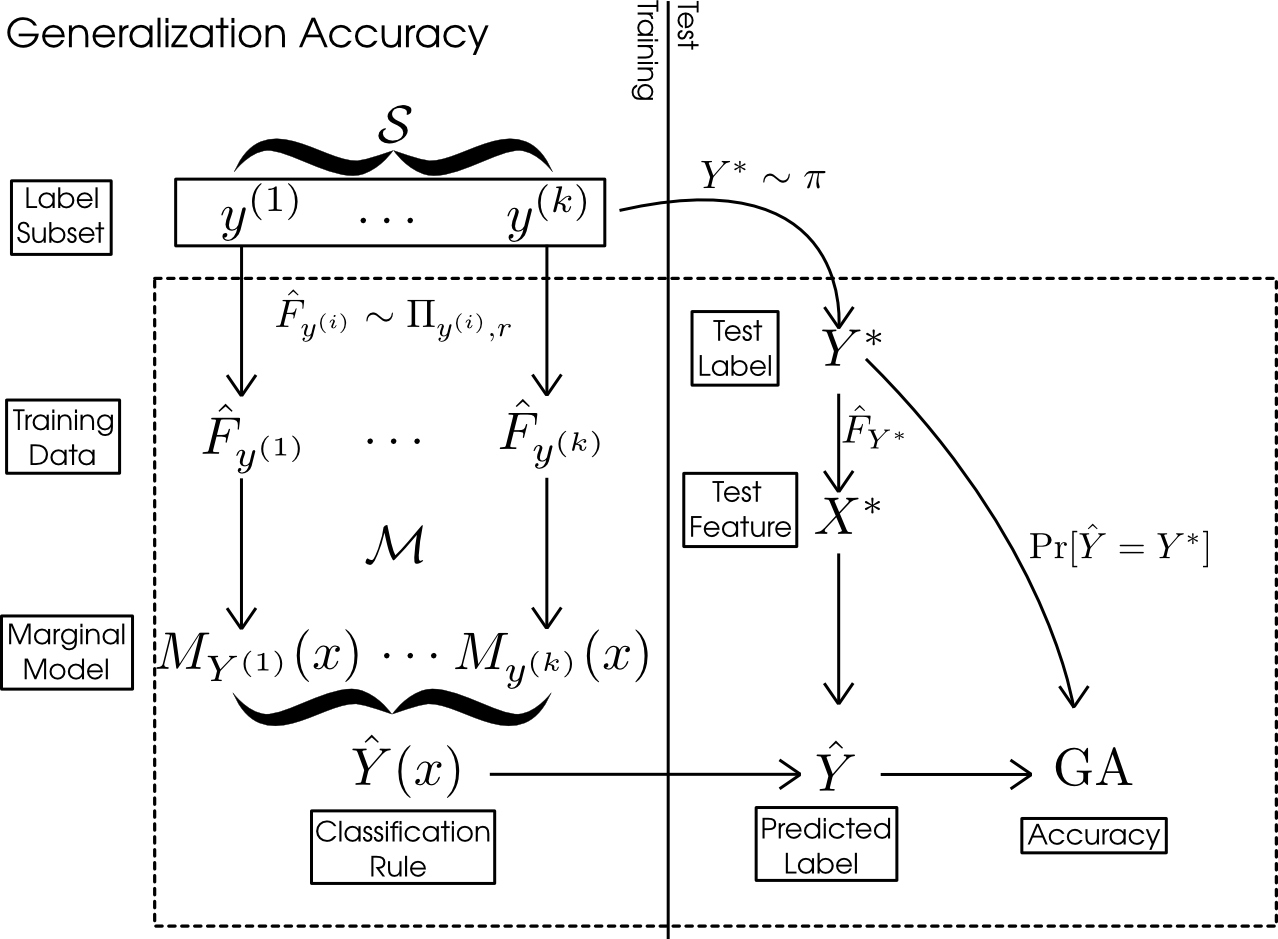
\includegraphics[scale = 0.3]{risk.png}
\caption{Generalization accuracy}\label{fig:risk}
\end{figure}

Finally, suppose we do not fix any of the random quantities in the
classification task $P$, and merely specify $k$, the number of
classes, and $r_1$, the number of repeats in the training set.  
Then the $k$-class, $r$-repeat \emph{average generalization accuracy} of
a marginal classifier $\mathcal{M}$ is defined as
\begin{align*}
\text{AGA}_{k,r_1}(\mathcal{M}) &= \E[\text{GA}_{\mathcal{S}}(\mathcal{M})|Y^{(1)}, \hdots, Y^{(k)} \sim \pi]
\\&= \frac{1}{k} \sum_{i=1}^k \int
I(\mathcal{M}(\hat{F}_{y^{(i)}})(x) = \max_j
\mathcal{M}(\hat{F}_{y^{(j)}})) dF_{y^{(i)}}(x) \prod_{\ell=1}^k
d\Pi_{y^{(\ell)}, r_1}(\hat{F}_{y^{(\ell)}}) d\pi(y^{(\ell)}).
\\&= \int
I(\mathcal{M}(\hat{F}_{y^{(1)}})(x) = \max_j
\mathcal{M}(\hat{F}_{y^{(j)}})) dF_{y^{(1)}}(x) \prod_{\ell=1}^k
d\Pi_{y^{(\ell)}, r_1}(\hat{F}_{y^{(\ell)}}) d\pi(y^{(\ell)}).
\end{align*}
where the last line follows from noting that all $k$ summands in the previous line are identical.
The definition of average generalization accuracy is illustrated in Figure \ref{fig:average_risk}.

\begin{figure}[h]
\centering
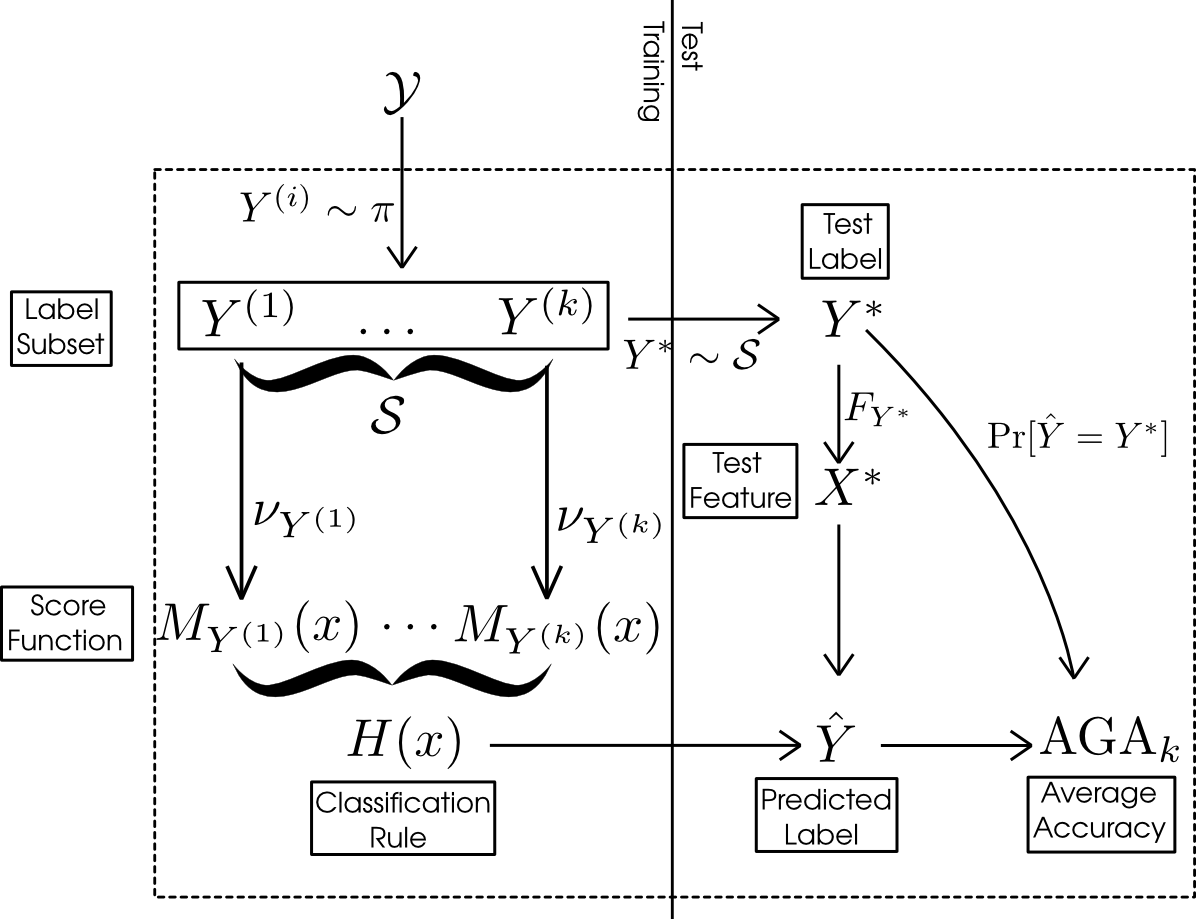
\includegraphics[scale = 0.3]{average_risk.png}
\caption{Average generalization accuracy}\label{fig:average_risk}
\end{figure}

Having defined the average (generalization) accuracy for the randomized classification
task, we begin to develop the theory of how to \emph{estimate} the
average accuracy in the next section.

\section{Estimation of average accuracy}\label{sec:estimation_average_accuracy}

Suppose we have training and test data for a classification task $P_1$
with $k_1$ classes, $r_1$-repeat training data and $r_2$-repeat test
data.  That is, we have label set $\mathcal{S}_1 =
\{y^{(i)}\}_{i=1}^{k_1}$, as well as training sample $\hat{F}_{y^{(i)}}$
and test sample $(x_1^{(i)},\hdots, x_{r_2}^{(i)})$ for $i =
1,\hdots, k_1$.  How can we estimate the $k, r$-average accuracy of a
marginal classifier $\mathcal{M}$ for arbitrary $k$ and $r$?

Let us start with the case $k = k_1$ and $r = r_1$.  Then the answer
is simple: construct the classification rule $h$ using marginal model
$\mathcal{M}$ from the training data.  Then the test accuracy of $h$ is an
unbiased estimator of $\text{AGA}_{k,r}$.

This follows from definition.  Observe that $\text{AGA}_{k_1,r_1}$ is
the expected prediction risk for the classification rule $h$ for a
randomized classification problem $P$ with $k_1$ classes and
$r_1$-repeat training data.  Of course, the classification task $P_1$
that we have been given is a random draw from the desired
distribution of random classification problems.  Therefore, the
prediction risk of $h$ constructed from $P_1$ is unbiased for
$\text{AGA}_{k_1, r_1}$, and since test accuracy is unbiased for
generalization accuracy, it follows that the test accuracy of $h$ is
an unbiased estimator of $\text{AGA}_{k,r}$, as we claimed.

In following sections, we consider more complicated cases where $k_1
\neq k$.  However, before proceeding, let us first review the
procedure for computing the test accuracy.

For any given test observation $x_j^{(i)}$, we obtain the predicted
label $\hat{y}_j^{(i)}$ by computing the margin for each class,
\[
M_{i,j,\ell} = \mathcal{M}(\hat{F}_{y^{(\ell)}})(x_j^{(i)}) =  m_{y^{(\ell)}}(x_i^{(j)}),
\]
for $\ell = 1,\hdots, k_1$,
and by finding the class with the highest margin $M_{i, j, \ell}$,
\[
\hat{y}_j^{(i)} = y^{(\argmax_\ell M_{i, j, \ell})}.
\]
The test accuracy is the fraction of correct classification over test observations,
\begin{equation}
\text{TA} = \frac{1}{r_2k_1} \sum_{i=1}^{k_1} \sum_{j=1}^{r_2} I(\hat{y}_j^{(i)} = y^{(i)}).
\end{equation}
For each test observation, define the ranks of the margins by
\[
R_{i,j,\ell} = \sum_{m \neq \ell} I\{M_{i,j,\ell} \geq M_{i, j, m}\}.
\]
Therefore, $\hat{y}_j^{(i)}$ is equal to $y^{(i)}$ if and only if $R_{i,j,i} = k_1$.
Thus, an equivalent expression for test accuracy is
\begin{equation}\label{eq:test_risk}
\text{TA} = \frac{1}{r_2 k_1} \sum_{i=1}^{k_1} \sum_{j=1}^{r_2} I\{R_{iji} = k_1\}.
\end{equation}

\subsection{Subsampling method}

Next, let us consider the case where $k < k_1$ and $r=r_1$.  Define a
classification problem $P_2$ with label set $\mathcal{S}_2$ obtained
by sampling $k$ labels uniformly without replacement from
$\mathcal{S}_1$.  Let the training and test data for $P_2$ be obtained
by taking the training data and test data from $P_1$ belonging to
labels in $\mathcal{S}_1$.  It follows that $P_2$ is a randomized
classification task with $k$ labels, $r_1$-repeat training data and
$r_2$-repeat test data.  Therefore, by the previous argument, the test
accuracy for a classification rule $h$ constructed using the training data
in $P_2$ provides an unbiased estimate of $\text{AGA}_{k, r_1}$.

However, we can get a much better unbiased estimate of
$\text{AGA}_{k, r_1}$ by averaging over the randomization of
$\mathcal{S}_2$.  Na\"{i}vely, this requires us to train and evaluate
${k_1}\choose{k}$ classification rules.  However, due to the special
structure of marginal classifiers, we do the computation in the same
order of computation as evaluating a single classification rule
(assuming that the computational bottleneck is in training the
classifier.)

This is because the rank $R_{iji}$ of the correct label, $i$, for the
$x_j^{(i)}$ allows us to determine how many subsets $\mathcal{S}_2$
will result in a correct classification.  For example $x_j^{(i)}$,
there are $R_{iji} - 1$ labels with a lower margin than the correct
label $i$.  Therefore, as long as one of the classes in
$\mathcal{S}_2$ is $i$, and the other $k-1$ labels are from the set of
$R_{iji}-1$ labels with lower margin than $i$, the classification of
$x_j^{(i)}$ will be correct.  This implies that there are
${R_{iji}-1}\choose{k-1}$ such subsets $\mathcal{S}_2$ where
$x_j^{(i)}$ is classified correctly, and therefore

\begin{equation}\label{eq:avtestrisk}
\text{AverageTA}_{k, r_1} = \frac{1}{{{k_1}\choose{k}}}\frac{1}{r_2 k} \sum_{i=1}^{k_1} \sum_{j=1}^{r_2} {{R_{iji}-1}\choose{k-1}}.
\end{equation}

\section{Extrapolation}

In this chapter, we continue the discussion of Chapter 2, but focus
specifically on the the question of how to estimate the $k$-class
average accuracy, $\text{AGA}_{k, r}$, based on data from a problem
$P_1$ with $k_1 < k$ classes, and $r = r_1$-repeat training data.
This problem of \emph{prediction extrapolation} is especially
interesting for a number of applied problems.

\begin{itemize} 
\item Example 1: A researcher develops a classifier for the purpose of labelling
images in 10,000 classes. However, for a pilot study, her resources are sufficient to 
tag only a smaller subset of these classes, perhaps 100. Can she estimate how well the algorithm 
work on the full set of classes based on an initial "pilot" subsample of class labels?
\item Example 2: A neuroscientist is interested in how well the brain
  activity in various regions of the brain can discriminate between
  different classes of stimuli.  \cite{Kay2008a} obtained fMRI brain
  scans which record how a single subject's visual cortex responds to
  natural images. They wanted to know how well the brain signals could
  discriminate between different images. For a set of 1750
  photographs, they constructed a classifier which achieved over 0.75
  accuracy of classification. Based on exponential extrapolation, they
  estimate that it would take on the order of $10^{9.5}$ classes
  before the accuracy of the model drops below 0.10!  A theory of
  performance extrapolation could be useful for the purpose of making
  such extrapolations in a more principled way.
\item The stories just described can be viewed as a metaphor for
  typical paradigm of machine learning research, where academic
  researchers, working under limited resources, develop novel
  algorithms and apply them to relatively small-scale datasets. Those
  same algorithms may then be adopted by companies and applied to much
  larger datasets with many more classes. In this scenario, it would
  be convenient if one could simply assume that performance on the
  smaller-scale classification problems was highly representative of
  performance on larger-scale problems.
\end{itemize}

Previous works have shown that generalizing from a small set of
classes to a larger one is not straightforward. In a paper titled
``What does classifying more than 10,000 Image Categories Tell Us,''
Deng and co-authors compared the performance of four different
classifiers on three different scales: a small-scale (1,000-class)
problem, medium-scale (7,404-class) problem, and large-scale
(10,184-class) problem (all from ImageNet.)  They found that while the
nearest-neighbor classifier outperformed the support vector machine
classifier (SVM) in the small and medium scale, the ranking switched
in the large scale, where the SVM classifier outperformed
nearest-neighbor.  As they write in their conclusion, ``we cannot
always rely on experiments on small datasets to predict performance at
large scale.'' Theory for performance extrapolation may therefore
reveal models with bad scaling properties in the pilot stages of
development.

However, in order to formally develop a method for extrapolating
performance, it is necessary to specify the model for how the
small-scale problem is related to the larger-scale problem.  The
framework of randomized classification introduced in Chapter 2 is one
possible choice for such a model: the small-scale problem and
large-scale problem are linked by having classes drawn from the same
population.

The rest of the chapter is organized as follows.  We begin by
continuing to analyze the average accuracy $\text{AGA}_{k, r}$, which
results in an explicit formula for the average accuracy.  The formula
reveals that all of the information needed to compute the average
accuracy is contained in a one-dimensional function $\bar{D}(u)$, and
therefore that estimation of the average accuracy can be accomplished
via estimation of the unknown function $\bar{D}(u)$.  This allows the
development of a class of unbiased estimators of $\bar{D}(u)$,
presented in section \ref{sec:extrapolation_estimation} given the
assumption of a known parametric form for $\bar{D}(u)$.  We analyze
the performance of the estimator in both the well-specified and
misspecified case.  We demonstrate our method to a face-recognition
example in section \ref{sec:extrapolation_example}.  Additionally, in
Chapter 5 %% cite the specific section later we will see the
comparison of the estimator to an alternative, information-theory
based estimator in simulated and real-data examples.

\subsection{Toy example}

Let us first illustrate using a toy example the computation of the
average risk, and preview the theory for extrapolating the average
risk.

Let $(Y, X)$ have a bivariate normal joint distribution,
\[
(Y, X) \sim N\left(\begin{pmatrix}0 \\0\end{pmatrix}, \begin{pmatrix}1 & \rho \\ \rho & 1\end{pmatrix}\right),
\]
as illustrated in figure \ref{fig:toy1}(a).
Therefore, for a given randomly drawn label $Y$, the conditional
distribution of $X$ for that label is univariate normal with mean $\rho Y$ and variance $1-\rho^2$:
\[
X|Y = y \sim N(\rho Y, 1-\rho^2).
\]
Supposing we draw $k = 3$ labels $y_1,y_2, y_3$, the classification
problem will be to assign a test instance $X^*$ to the correct label.
The test instance would be drawn from the three-class mixture,
\[
X^* \sim \frac{1}{k}\sum_{i=1}^k p(x|y_i),
\]
as illustrated in figure \ref{fig:toy1}(b, top).  In this toy example, we
ignore the issue of training a classifier from sampled data, and
instead assume that we have access to the \emph{Bayes classification
rule}, or optimal classification rule.  The Bayes rule assigns $X^*$
to the class with the highest density $p(x|y_i)$, as illustrated by
figure \ref{fig:toy1}(b, bottom).

\begin{figure}[h]
\centering
\begin{tabular}{cc}
\multirow{3}{*}{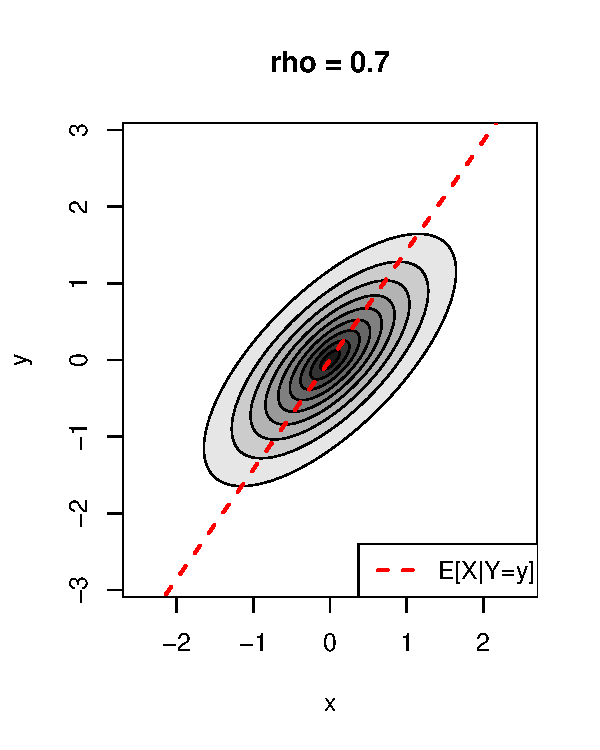
\includegraphics[scale = 0.5, clip = true, trim = 0 0 0 0.5in]{illus_rho_0_7.pdf}} & \\
& 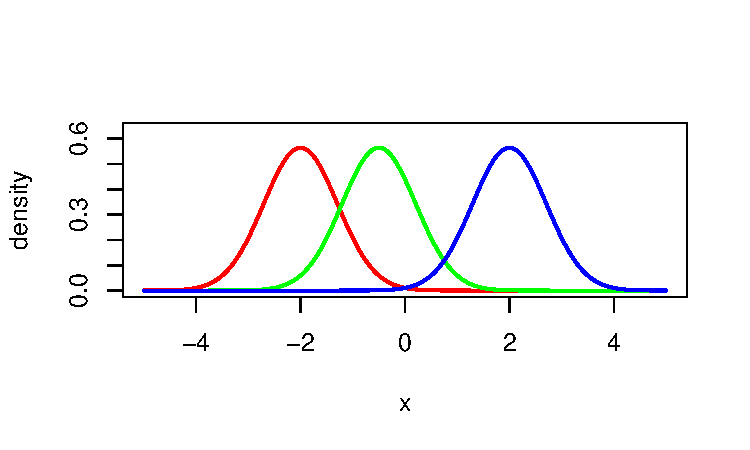
\includegraphics[scale = 0.5, clip = true, trim = 0 0.8in 0 0.8in]{illus_example1a.pdf}\\
 &  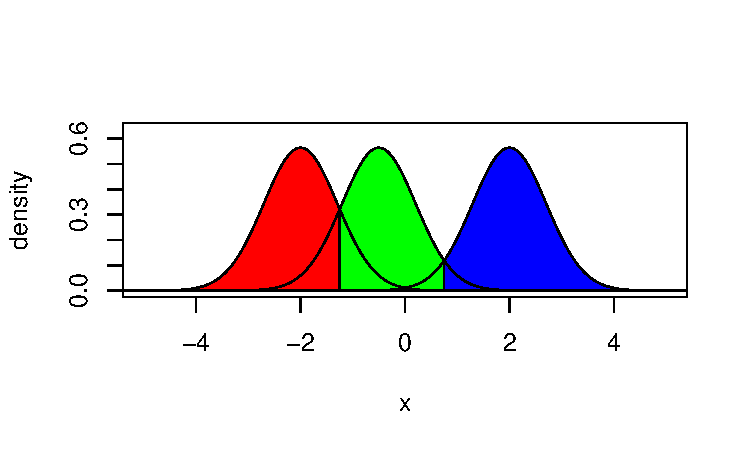
\includegraphics[scale = 0.5, clip = true, trim = 0 0 0 0.5in]{illus_example1b.pdf}\\
(a) & (b)
\end{tabular}

\caption{
(a) The joint distribution of $(X, Y)$ is bivariate normal with correlation $\rho = 0.7$.
(b) A typical classification problem instance from the bivariate normal model with $k = 3$ classes.
Top: the conditional density of $X$ given label $Y$, for $Y = \{y_1, y_2, y_3\}$.
Bottom: the Bayes classification regions for the three classes.}\label{fig:toy1}
\end{figure}

The risk of the Bayes rule for any label set $\{y_1,\hdots, y_k\}$ is given by
\[
\text{Risk}(y_1,\hdots, y_k) = \frac{1}{k}\sum_{i=1}^k \Pr_{X \sim p(x|y_i)}[p(X|y_i) = \max_{j=1}^k p(X|y_j)].
\]
We numerically computed $\text{Risk}(y_1,\hdots, y_k)$ for randomly
drawn labels $Y_1,\hdots, Y_k \stackrel{iid}{\sim} N(0, 1)$; the
distributions of $\text{Risk}(Y_1,\hdots, Y_k)$ for $k = 2,\hdots, 10$
are illustrated in figure \ref{fig:toy2}.  The $k$-class average risk,
$\text{AvRisk}_k$, in this case, is given by
\[
\text{AvRisk}_k = \E[\text{Risk}(Y_1,\hdots, Y_k)]
\]
for $Y_1,\hdots, Y_k \stackrel{iid}{\sim} N(0, 1)$. The theory
presented in the rest of the section deals with how to analyze the
average risk $\text{AvRisk}_k$ as a function of $k$.  We now proceed
to preview some selected aspects of the theory for the toy example.

\begin{figure}[h]
\centering
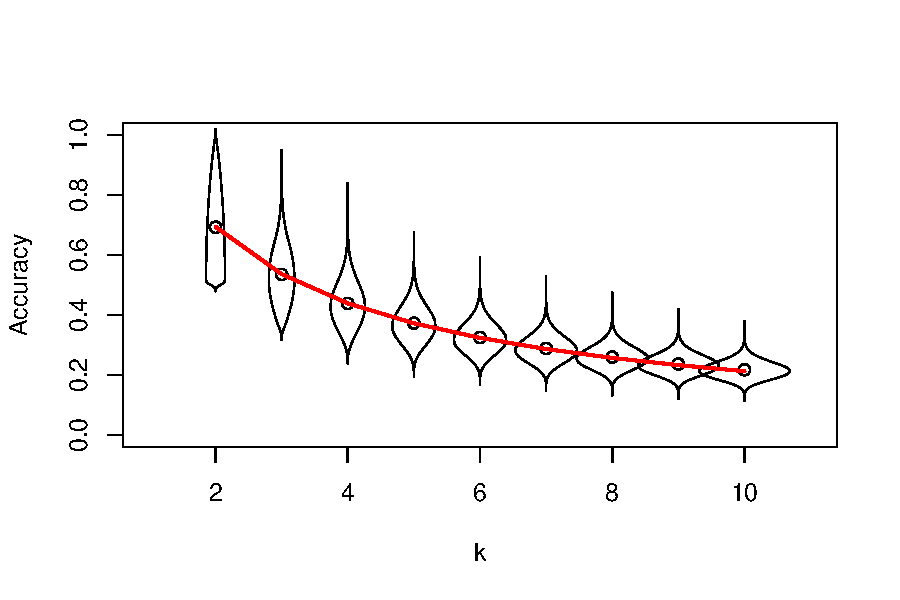
\includegraphics[scale = 0.7, clip = true, trim = 0 0 0 0.5in]{illus_err_0_7.pdf}

\caption{The distribution of the classification risk for $k = 2,3,\hdots, 10$ for the bivariate normal model with $\rho = 0.7$.
Circles indicate the average classificatin risk; the red curve is the theoretically computed average risk.}\label{fig:toy2}
\end{figure}

For a given test instance $X^*$ drawn from the label $Y^*$, the closer
that $X^*$ is to the center of the correct class distribution, $\rho
Y^*$, the more likely it is to be classified correctly.  Based on this
concept, we define the \emph{conditional accuracy} function $U_x(y)$,
which gives the conditional probability that a test instance $(Y_1,
X_1)$ will be classified correctly in the two-class classification
problem.  One can therefore think of $U_x(y)$ as measuring the
``strength'' of the pair $(y, x)$, with stronger pairs being more
likely to be classified correctly.  Since in the two-class problem,
there is one incorrect class label $Y_2$, the conditional accuracy in
this case is simply the probability that $\rho Y_2$ is closer to $X_1$
than $\rho Y_1$.  Therefore, in this toy example, we can give an
explicit formula
\begin{align*}
U_x(y) &= \Pr[p(x|y) < p(x|Y)]
\\&= \Pr[|\rho Y - x|< |\rho y - x|] 
\\&= \Phi\left(\frac{x + |\rho y - x|}{\rho}\right) - \Phi\left(\frac{x - |\rho y - x|}{\rho}\right),
\end{align*}
where $\Phi$ is the standard normal cumulative distribution function.
Figure \ref{fig:toy3}(a) illustrates the level sets of the function
$U_x(y)$.  The highest values of $U_x(y)$ are near the line $x = \rho
y$ corresponding the to conditional mean of $X|Y$: as one moves
farther from the line, $U_x(y)$ decays.  Note however that large
values of $(y, x)$ (with the same sign) result in larger values of
$U_x(y)$ since it becomes unlikely for $Y_2 \sim N(0,1)$ to exceed
$Y_1 = y$.

Now define the random variable $U = U_X(Y)$ for $(X, Y)$ drawn from
the joint distribution.  An important object in our theory is the
cumulative distribution function
\footnote{Note however that $\bar{D}(u)$ is only defined as the cumulative
distribution function of $U$ in the class of zero-one loss--the
definition for general cost functions is somewhat more involved, as we
will see.}
of $U$, written as
\[
\bar{D}(u) = \Pr[U \leq u].
\]
The function $\bar{D}$ is illustrated in
figure \ref{fig:toy3}(b) for the current example with $\rho = 0.7$.
The red curve in figure \ref{fig:toy2} was computed using the formula
\[
\text{AvRisk}_k = (k-1) \int \bar{D}(u) u^{k-2} du.
\]

\begin{figure}[h]
\centering
\begin{tabular}{cc}
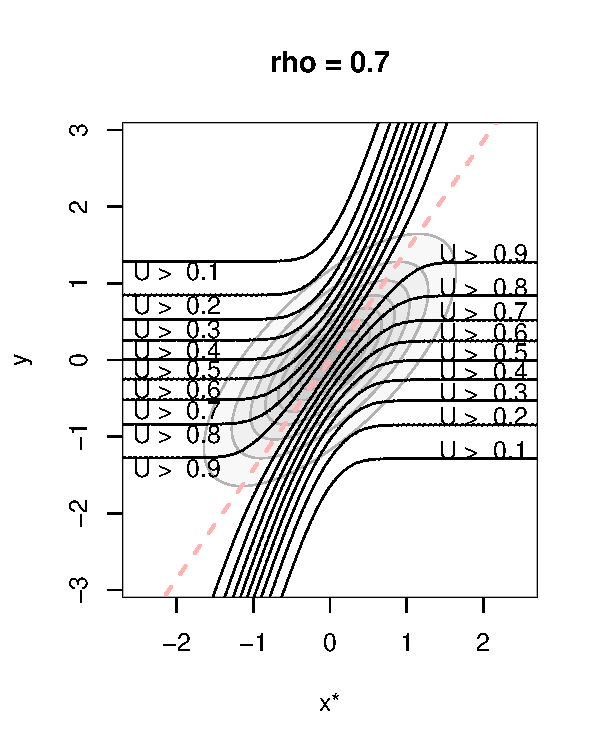
\includegraphics[scale = 0.6, clip = true, trim = 0.1in 0 0 0.8in]{illus_ufunc_0_7.pdf} &
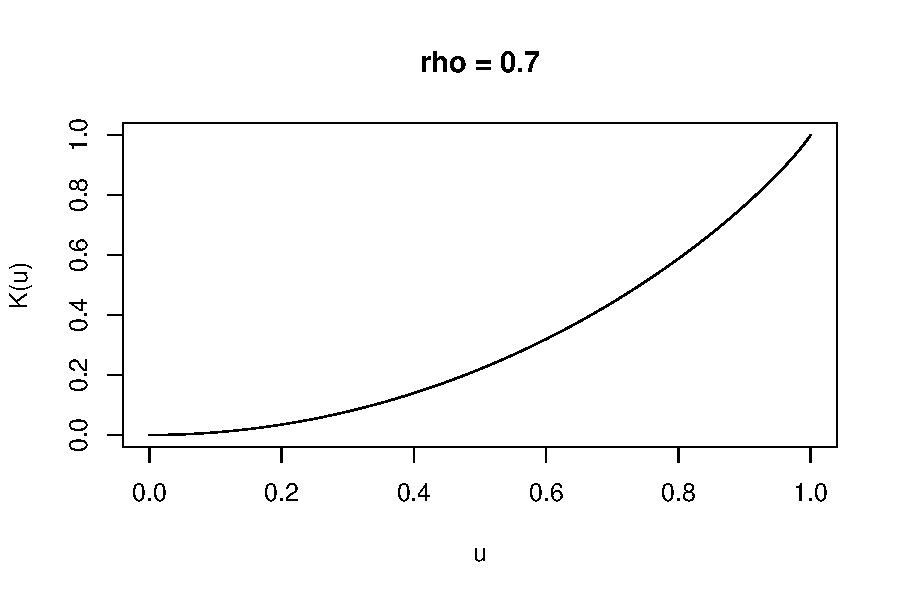
\includegraphics[scale = 0.65, clip = true, trim = 0 -0.3in 0 0.5in]{illus_kfunc_0_7.pdf}\\
(a) & (b)
\end{tabular}

\caption{
(a) The level curves of the function $U_x(y)$ in the bivariate normal model with $\rho = 0.7$.
(b) The function $\bar{D}(u)$, which gives the cumulative distribution function of the random variable $U_Y(X)$.}\label{fig:toy3}
\end{figure}

It is illuminating to consider how the average risk curves and the
$\bar{D}(u)$ functions vary as we change the parameter $\rho$.  Higher
correlations $\rho$ lead to lower classification risk, as seen in
figure \ref{fig:toy4}(a), where the risk curves are shifted downward as
$\rho$ increases from 0.3 to 0.9.  The conditional accuracy $U_y(x)$
tends to be higher on average as well, which leads to lower values of
the cumulative distribution function--as we see in
figure \ref{fig:toy4}(b), where the function $\bar{D}(u)$ becomes smaller
as $\rho$ increases.

In section \ref{sec:estimation}, when we consider approximating
$\bar{D}(u)$ by polynomials, or some other function basis, it becomes
relevant to consider how well $\bar{D}(u)$ can be approximated by such
bases in realistic problems.  We see in figure \ref{fig:toy4}(c) that,
at least in this toy problem, $\bar{D}(u)$ is well-aproximated by
low-order polynomials.  However, the approximation becomes less
adequate as $\rho$ increases.  We can see visually why this is the
case: as $\rho$ increases, the curvature of $\bar{D}(u)$ near $u = 1$
increases.  Hence, higher-degree polynomials become needed to capture
the behavior near $u = 1$.  More generally, we observe that in cases
where classes are relatively well-separated, it becomes necessary to
use increasingly precise approximations in order to extrapolate the
average risk.

\begin{figure}[h]
\centering
\begin{tabular}{ccc}
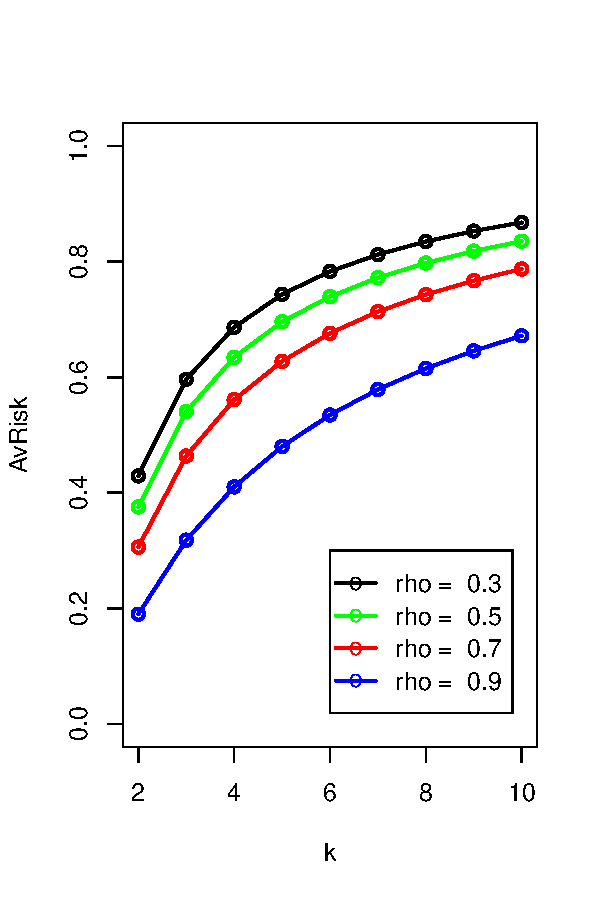
\includegraphics[scale = 0.45, clip = true, trim = 0.05in 0 0.2in 0.6in]{illus_rhos_avrisk.pdf} &
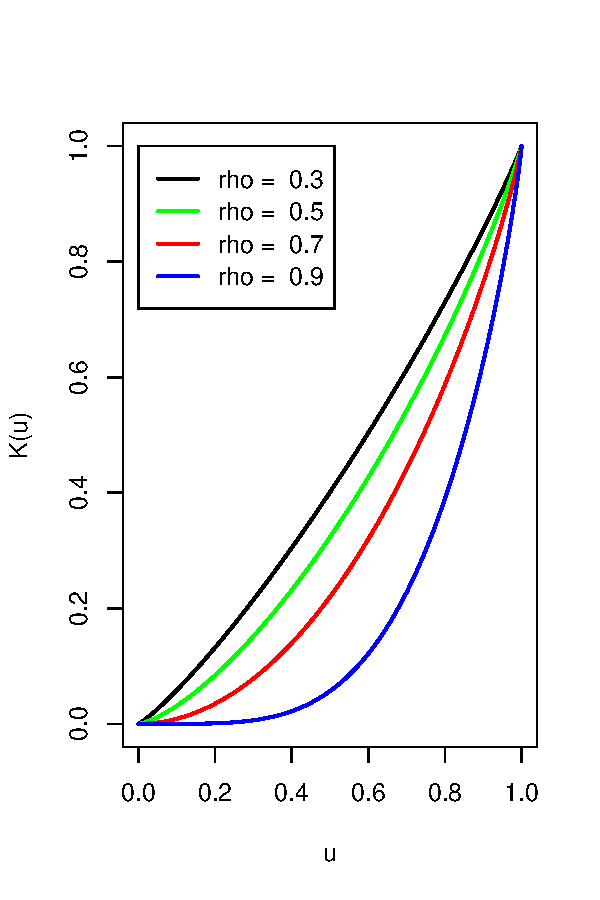
\includegraphics[scale = 0.45, clip = true, trim = 0.05in 0 0.2in 0.6in]{illus_rhos_Kfunc.pdf} &
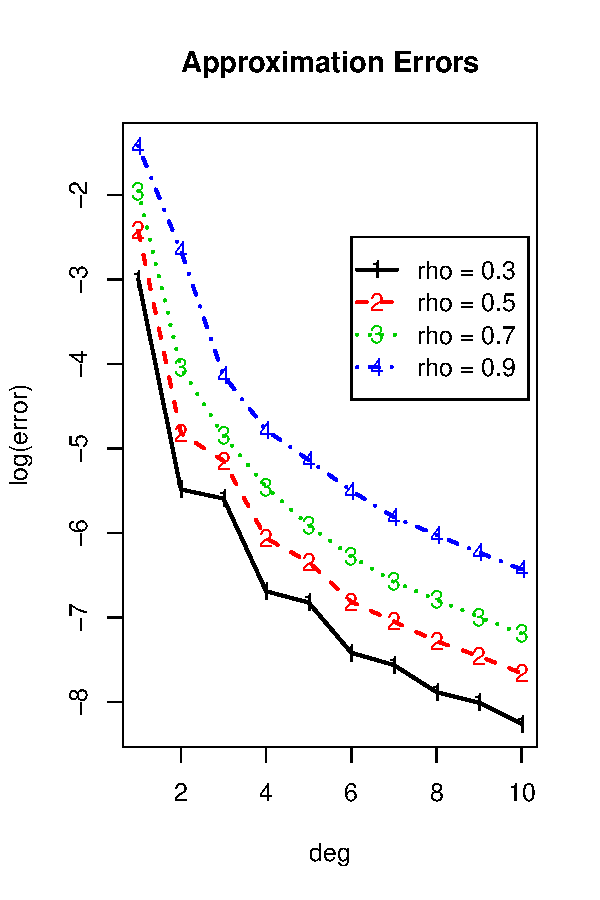
\includegraphics[scale = 0.45, clip = true, trim = 0.05in 0 0.2in 0.6in]{illus_approx_errors.pdf}\\
(a) & (b) & (c)
\end{tabular}

\caption{
The (a) average risk, (b) $\bar{D}(u)$ function for $k = 2,\hdots, 7$ for the bivariate normal model with $\rho \in \{0.3, 0.5, 0.7, 0.9\}$.
(c) The $d$-degree $\ell_\infty$ polynomial approximation error for $\bar{D}(u)$ for the bivariate normal model with $\rho \in \{0.3, 0.5, 0.7, 0.9\}$.
}\label{fig:toy4}
\end{figure}

\subsection{Analysis of average risk}

The result of our analysis is to expose the average accuracy
$\text{AGA}_{k, r}$ as the weighted average of a function
$\bar{D}(u)$, where $\bar{D}(u)$ is independent of $k$, and where $k$
only changes the weighting.  The result is stated as follows.

\begin{theorem}\label{theorem:avrisk_identity}
Suppose $\pi$, $\{F_y\}_{y \in \mathcal{Y}}$ and marginal classifier
$\mathcal{F}$ satisfy the tie-breaking condition.  Then, under the
definitions \eqref{eq:U_function} and \eqref{eq:Kbar}, we have
\begin{equation}\label{eq:avrisk_identity}
\text{AGA}_{k, r} = 1 - (k-1) \int \bar{D}(u) u^{k-2} du.
\end{equation}
\end{theorem}

The tie-breaking condition referred in the theorem is defined as follows.
\begin{itemize}
\item 
\emph{Tie-breaking condition}: for all $x \in \mathcal{X}$,
$\mathcal{M}(\hat{F}_Y)(x) = \mathcal{M}(\hat{F}_{Y'})(x)$
with zero probability for $Y, Y'$ independently drawn from $\pi$.
\end{itemize}
The tie-breaking condition is a technical assumption which allows us
to neglect the specification of a tie-breaking rule in the case that
margins are tied.  In practice, one can simply break ties randomly,
which is mathematically equivalent to adding a small amount of random
noise $\epsilon$ to the function $\mathcal{M}$.

As we can see from Figure \ref{fig:average_risk}, the average accuracy is
obtained by averaging over four randomizations:
\begin{enumerate}
\item[A1.] Drawing the label subset $\mathcal{S}$.
\item[A2.] Drawing the training dataset.
\item[A3.] Drawing $Y^*$ uniformly at random from $\mathcal{S}$.
\item[A4.] Drawing $X^*$ from $F_{X^*}$.
\end{enumerate}


Our strategy is to analyze the average accuracy by
means of \emph{conditioning on} the true label and its training
sample, $(y^*, \hat{F}_{y^*})$, and the test feature $x^*$
while \emph{averaging} over all the other random variables.  Define
the \emph{conditional accuracy} $\text{CondAcc}_k((y^*, \hat{F}_{y^*}), x^*)$ as
\[
\text{CondAcc}_k((y^*, \hat{F}_{y^*}), x^*) = \Pr[\argmax_{y \in \mathcal{S}} \mathcal{M}(\{\hat{F}_y\})(X^*) = Y^* |Y^*=y^*, X^* = x^*, \hat{F}_{Y^*} = \hat{F}_{y^*}].
\]
Figure \ref{fig:conditional_risk} illustrates the variables which are
fixed under conditioning and the variables which are randomized.
Compare to figure \ref{fig:average_risk}.

Without loss of generality, we can write the label subset $\mathcal{S}
= \{Y^*, Y^{(1)},\hdots, Y^{(k-1)}\}$.  Note that due to independence,
$Y^{(1)},\hdots, Y^{(k-1)}$ are still i.i.d. from $\pi$ even
conditioning on $Y^* = y^*.$ Therefore, the conditional risk can be
obtained via the following alternative order of randomizations:
\begin{enumerate}
\item[C0.] 
Fix $y^*, \hat{F}_y^*,$ and $x^*$.  Note that $M_{y^*}(x^*)
= \mathcal{M}(\hat{F}_{y^*})(x^*)$ is also fixed.
\item[C1.]
Draw the \emph{incorrect labels} $Y^{(1)},\hdots, Y^{(k)}$ i.i.d. from
$\pi$.  (Note that $Y^{(i)} \neq y^*$ with probability 1 due to the
continuity assumptions on $\mathcal{Y}$ and $\pi$.)
\item[C2.]
Draw the training samples for the incorrect labels
$\hat{F}_{Y^{(1)}},\hdots, \hat{F}_{Y^{(k-1)}}$.  This determines
\[
\hat{Y} = \argmax_{y \in \mathcal{S}} M_y(x^*)
\]
and hence, whether or not the classification is correct for $(x^*, y^*)$
\end{enumerate}
Compared to four randomization steps for the average risk, we have
essentially conditioned on steps A3 and A4 and randomized over steps
A1 and A2.

\begin{figure}[h]
\centering
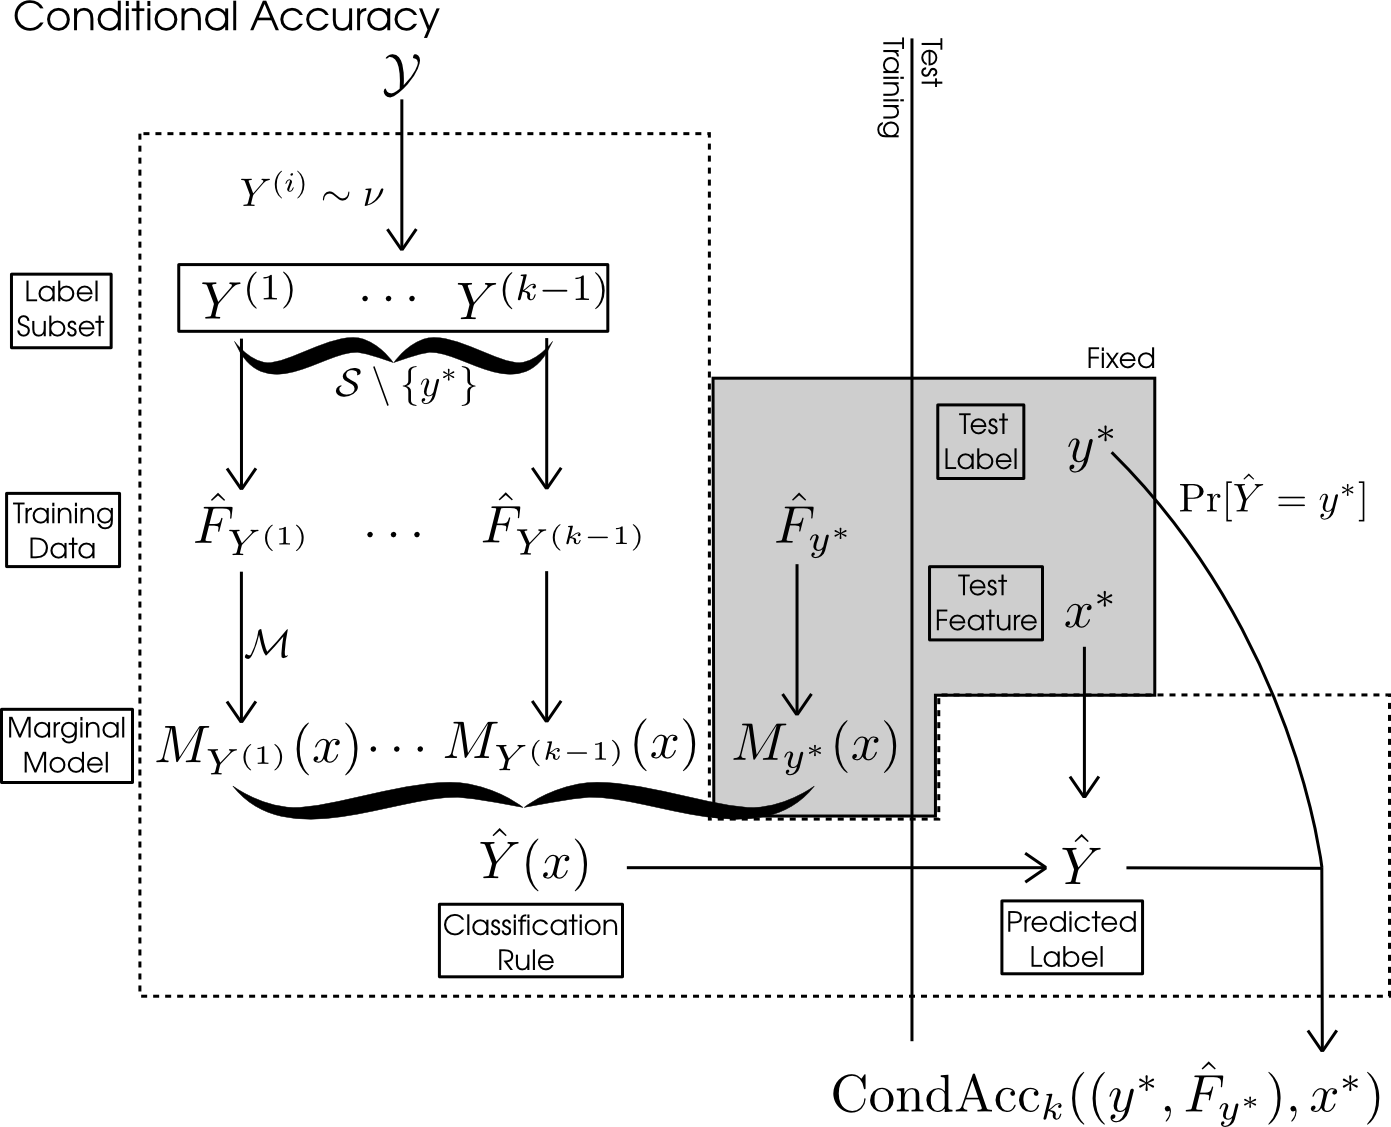
\includegraphics[scale = 0.3]{conditional_risk.png}
\caption{Conditional accuracy}\label{fig:conditional_risk}
\end{figure}

Now, in order to analyze the $k$-class behavior of the conditional
accuracy, we begin by considering the \emph{two-class} situation.

In the two-class situation, we have a true label $y^*$, a training
sample $\hat{F}_{y^*}$, and one incorrect label, $Y$.  Define the
\emph{U-function} $U_{x^*}(y^*, \hat{F}_{y^*})$ as the conditional
accuracy (the probability of correct classification) in the two-class
case.  The classification is correct if the margin $M_{y^*}(x^*)$ is
greater than the margin $M_Y(x^*)$, and incorrect otherwise.  Since we
are fixing $x^*$ and $(y^*, \hat{F}_{y^*})$, the probability of
correct classification is obtained by taking an expectation:
\begin{align}\label{eq:U_function}
U_{x^*}(y^*, \hat{F}_{y^*}) &= \Pr[M_{y^*}(x^*) > \mathcal{M}(\hat{F}_Y)(x^*)]
\\&= \int_{\mathcal{Y}} 
I\{
M_{y^*}(x^*) > \mathcal{M}(\hat{F}_{y})(x)
\}
d\Pi_{y, r}(\hat{F}_y)
d\pi(y).
\end{align}
See also figure \ref{fig:U_function} for an graphical illustration of
the definition.

\begin{figure}[h]
\centering
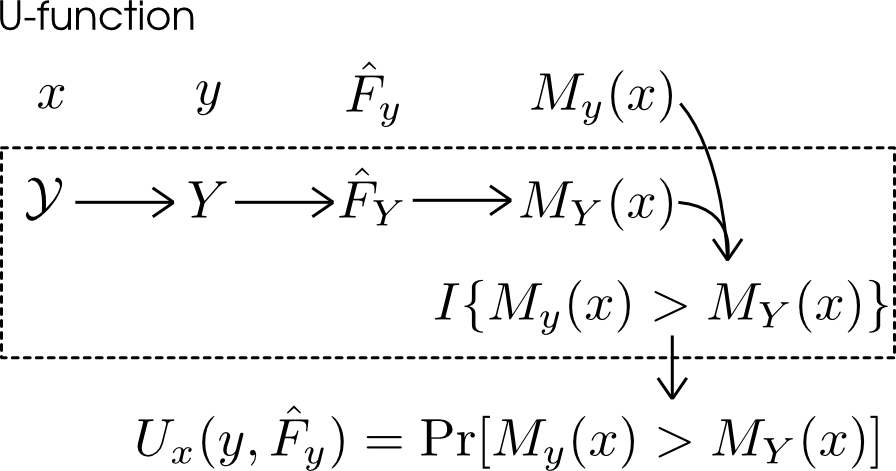
\includegraphics[scale = 0.4]{U_function.png}
\caption{U-functions}\label{fig:U_function}
\end{figure}

An important property of the U-function, and the basis for its name,
is that the random variable $U_x(Y, \hat{F}_Y)$ for $Y \sim \pi$ and
$\hat{F}_Y \sim \Pi_{Y, r}$ is uniformly distributed for all
$x \in \mathcal{X}$.  This is proved in Lemma \ref{lemma:U_function}
in Appendix C.

Now, we will see how the U-function allows us to understand the
$k$-class case.  Suppose we have true label $y^*$ and incorrect labels
$Y^{(1)},\hdots, Y^{(k-1)}$.  Note that the U-function
$U_{x^*}(y, \hat{F}_y)$ is monotonic in $M_y(x^*)$.  Therefore,
\[
\hat{Y} = \argmax_{y \in \mathcal{S}} M_y(x^*) = \argmax_{y \in \mathcal{S}} U_{x^*}(y, \hat{F}_y).
\]
Therefore, we have a correct classification if and only if the U-function value for the correct label
is greater than the maximum U-function values for the incorrect labels:
\[
\Pr[\hat{Y} = y^*] = \Pr[U_{x^*}(y^*, \hat{F}_{y^*}) > \max_{i=1}^{k-1} U_{x^*}(Y^{(i)}, \hat{F}_{Y^{(i)}})] =  \Pr[u^* > U_{max}].
\]
where $u^* = U_{x^*}(y^*, \hat{F}_{y^*})$ and $U_{max, k-1}
= \max_{i=1}^{k-1} U_{x^*}(Y^{(i)}, \hat{F}_{Y^{(i)}})$.  But now,
observe that we know the distribution of $U_{max, k-1}$!  Since
$U_{x^*}(Y^{(i)}, \hat{F}_{Y^{(i)}})$ are i.i.d. uniform, we know that
\begin{equation}\label{eq:umax_beta}
U_{max, k-1} \sim \text{Beta}(k-1, 1). 
\end{equation}

Therefore, in the general case, the conditional accuracy is
\[
\text{CondAcc}_k((y^*, \hat{F}_{y^*}), x^*) = \Pr[U_{max} > u^*] = 1 - \int_{u^*}^1 (k-1) u^{k-2} du.
\]
Now the average accuracy can be obtained by integrating over the
distribution of $U^* = U_{x^*}(y^*, \hat{F}_{y^*})$, which we state in
the following proof of theorem \ref{theorem:avrisk_identity}.

\noindent\textbf{Proof of Theorem \ref{theorem:avrisk_identity}}.
We have
\begin{align*}
\text{AGA}_{k,r} &= \E[ 1 - \int_{U^*}^1 (k-1) u^{k-2} du] 
\\&= 1 - \E[\int_0^1 I\{u \geq U^*\} (k-1) u^{k-2} du ]
\\&= (k-1) \int_0^1 \Pr[U^* \leq u] u^{k-2} du.
\end{align*}
Or equivalently,
\[
\text{AGA}_{k, r}((y^*, \hat{F}_{y^*}), x^*) = 1 - (k-1) \int \bar{D}(u) u^{k-2} du.
\]
where $\bar{D}(u)$ denotes the cumulative distribution function of $U^*$ on $[0,1]$:
\begin{equation}\label{eq:Kbar}
\bar{D}(u) = \Pr[U_{x^*}(y^*, \hat{F}_{y^*}) \leq u].
\end{equation}
We have expressed the average risk expressed as a weighted integral of
a certain function $\bar{D}(u)$ defined on $u \in [0,1]$.  We have
clearly isolated the part of the average risk which is independent of
$k$--the univariate function $\bar{D}(u)$, and the part which is
dependent on $k$--which is the density of $U_{max}$.

In section \ref{sec:extrapolation_estimation}, we will develop
estimators of $\bar{D}(u)$ in order to estimate the $k$-class average
risk.

Having this theoretical result allows us to understand how the
expected $k$-class risk scales with $k$ in problems where all the
relevant densities are known.  However, applying this result in
practice to estimate $\text{Average Risk}_k$ requires some means of
estimating the unknown function $\bar{D}$--which we discuss in the
following.

\subsection{Estimation}\label{sec:extrapolation_estimation}

Now we address the problem of estimating $\text{AGA}_{k_2, r_1}$ from
data.  As we have seen from Theorem \ref{theorem:avrisk_identity}, the
$k$-class average accuracy of a marginal classifier $\mathcal{M}$ is a
functional of a object called $\bar{D}(u),$ which depends marginal
model $\mathcal{M}$ of the classifier, the joint distribution of
labels $Y$ and features $X$ when $Y$ is drawn from the sampling
density $\nu$.

Therefore, the strategy we take is to attempt to estimate $\bar{D}$
for then given classification model, and then plug in our estimate of
$\bar{D}$ into the integral \eqref{eq:avrisk_identity} to obtain an
estimate of $\text{AGA}_{k_2, r_{train}}$.

Having decided to estimate $\bar{D}$, there is then the question of
what kind of model we should assume for $\bar{D}$.  In this work, we
assume that some parametric model\footnote{While a
nonparametric approach may be more ideal, we leave this to future work.} is available for $\bar{D}$.

Let us assume the linear model
\begin{equation}\label{eq:linearKu}
\bar{D}(u) = \sum_{\ell = 1}^m \beta_\ell h_\ell(u),
\end{equation}
where $h_\ell(u)$ are known basis functions, and $\beta$ are the model
parameters to be estimated. We can obtain \emph{unbiased} estimation
of $\text{AGA}_{k_2, r_{train}}$ via the unbiased estimates of
$k$-class average risk obtained from \eqref{eq:avtestrisk}.

If we plug in the assumed linear model \eqref{eq:linearKu} into the
identity \eqref{eq:avrisk_identity}, then we get
\begin{align}
1 - \text{AGA}_{k, r_{train}} &= 1 - (k-1)\int \bar{D}(u) u^{k-2} du
\\&= 1 - (k-1)\int_0^1 \sum_{\ell = 1}^m \beta_\ell h_\ell(u) u^{k-2} du
\\&= 1 - \sum_{\ell = 1}^m \beta_\ell H_{\ell,k} \label{eq:avrisk_linear}
\end{align}
where
\begin{equation}
H_{\ell,k} = (k-1) \int_0^1 h_\ell(u) u^{k-2} du.
\end{equation}
The constants $H_{\ell, k}$ are moments of the basis function
$h_\ell$: hence we call this method the \emph{moment method.}  Note
that $H_{\ell, k}$ can be precomputed numerically for any $k \geq 2$.


Now, since the test accuracies $\text{TA}_k$ are unbiased estimates of
$\text{AGA}_{k, r_{train}}$, this implies that the regression
estimate
\[
\hat{\beta} = \argmin_\beta \sum_{k=2}^{k_1} w_k \left( (1 - \text{TA}_k) - \sum_{\ell=1}^m \beta_\ell H_{\ell, k}\right)^2
\]
is unbiased for $\beta$, under any choice of positive weights $w_k$.
The estimate of $\text{AGA}_{k_2,r_1}$ is similarly obtained
from \eqref{eq:avrisk_linear}, via
\begin{equation}\label{eq:avrisk_hat}
\widehat{\text{AGA}_{k_2,r_1}} = 1 - \sum_{\ell=1}^m \hat{\beta}_\ell H_{\ell, k_2}.
\end{equation}

\section{Examples}\label{sec:extrapolation_example}

\subsection{Facial recognition example}

From the ``Labeled Faces in the Wild'' dataset (\cite{LFWTech}), we
selected 1672 individuals with at least 2 face photos.  We form a
dataset consisting of photo-label pairs $(\vec{z}_j^{(i)}, y^{(i)})$
for $i = 1,\hdots, 1672$ and $j = 1,2$ by randomly selecting 2 face
photos for each of the 1672 individuals.

We implement a face recognition system based on one nearest-neighbor
and OpenFace (\cite{amos2016openface}) for feature extraction.  For
each photo $\vec{z}$, a 128-dimensional feature vector $\vec{x}$ is
obtained as follows.
\begin{enumerate}
\item The computer vision library DLLib is used to detect landmarks in
  $\vec{z}$, and to apply a nonlinear transformation to align
  $\vec{z}$ to a template.
\item The aligned photograph is downsampled to a $96 \times 96$ input,
  which is fed into a pre-trained deep convolutional neural network to
  obtain the 128-dimensional feature vector $\vec{x}$.
\end{enumerate}
Therefore, we obtain feature-label pairs $(\vec{z}_j^{(i)}, y^{(i)})$
for $i = 1,\hdots, 1672$ and $j = 1,2$.

The recognition system then works as follows.  Suppose we want to
perform facial recognition on a subset of the individuals, $I \subset
\{1,\hdots, 1672\}$.  Then, for all $i \in I$, we load one feature
vector-label pair, into the system, $(\vec{x}_1^{(i)}, y^{(i)})$.  In
order to identify a new photo $\vec{z}^*$, we obtain the feature
vector $\vec{x}^*$, and guess the label $\hat{y}$ based on example
with the minimal distance to $\vec{x}^*$,
\[
\hat{y} = y^{(i^*)}
\]
where
\[
i^* = \text{argmin}_I d(\vec{x}, \vec{x}_1^{(i)}).
\]
The test accuracy is assessed on the unused repeat for all individuals
in $I$.  Note that the assumptions of our estimation method are met in
this example because one-nearest neighbor is a marginal classifier.
One can define the margin functions as
\[
(\mathcal{M}(\vec{x}))(\vec{x}^*) = -||\vec{x} - \vec{x}^*||^2.
\]
However, $k$-nearest neighbor for $k > 1$ is not marginal.

While we can apply our extrapolation method to estimate the average
accuracy for any number of faces $k$, it will not be possible to
validate our estimates if we use the full dataset.  Therefore, we take
the average accuracies computed using the subsampling method
\eqref{eq:avtestrisk} on the full dataset as a \emph{ground truth} to
compare to the average accuracy estimated from a \emph{subsampled}
dataset.  Therefore, we simulate the problem of performance
extrapolation from a database of $K$ faces by subsampling a
dataset of size $K$ from the LFW dataset.

\begin{figure}
\centering
\begin{tabular}{cc}
a & b\\
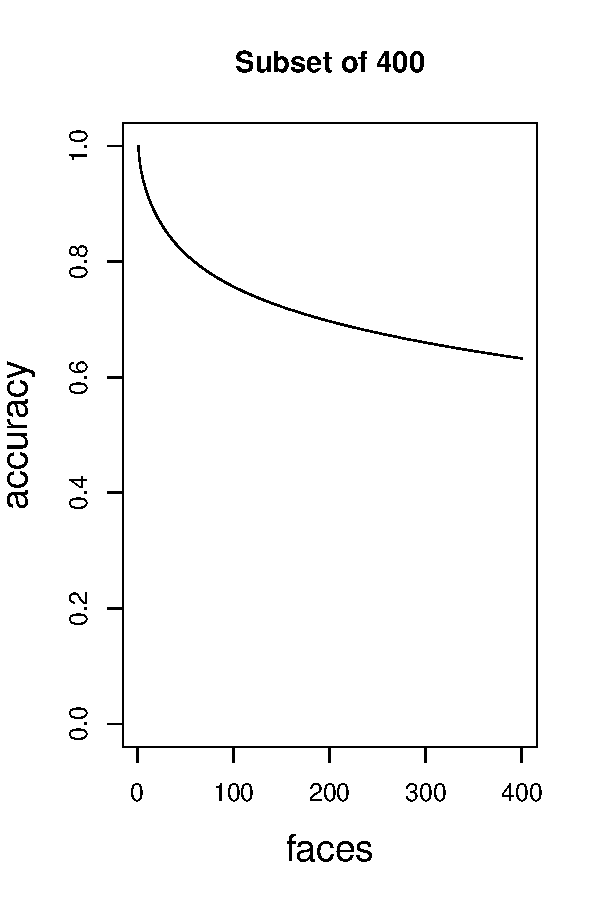
\includegraphics[scale = 0.5]{acc_plot1.pdf} &
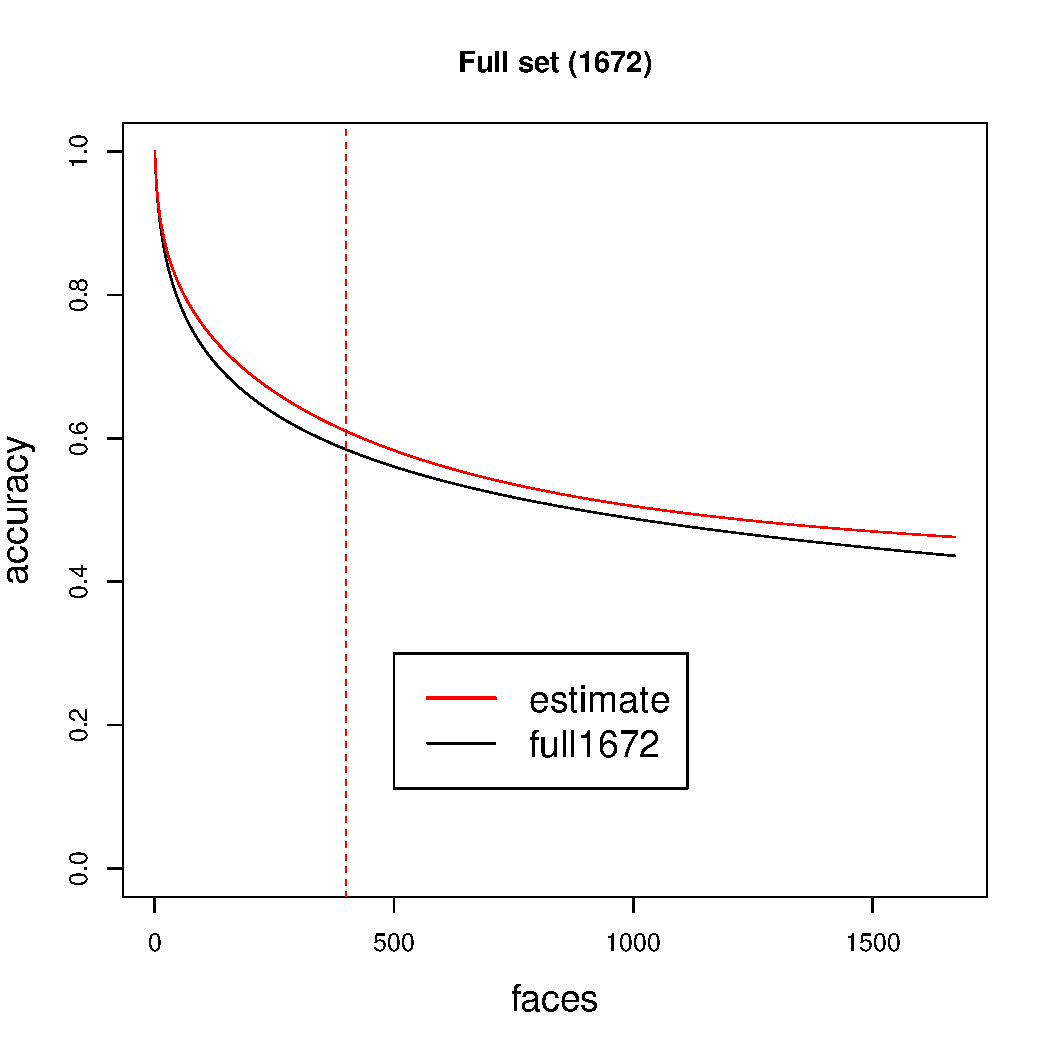
\includegraphics[scale = 0.5]{acc_plot2.pdf}
\end{tabular}
\caption{(a) The estimated average accuracy for $k = 2,\hdots,
  400$ given a dataset of 400 faces subsampled from Labeled Faces in
  the Wild.  (b) Estimated average accuracy for $k > 400$ on the
  same dataset, compared to the ground truth (average $k$-class test accuracy
  using all 1672 classes).}
\label{fig:lfw_extrapolation1}
\end{figure}

To do the performance extrapolation, we use a linear
spline basis,
\[
h_\ell(u) = \left[u - \frac{\ell - 1}{m}\right]_+
\]
for $\ell = 1,\hdots, m$.  Here we take $m = 10000$.  We model the
function $\bar{D}(u)$ as a non-negative linear combination of basis
functions,
\[
\bar{D}(u) = \sum_{\ell = 1}^m \beta_\ell h_\ell(u),
\]
with $\beta_\ell \geq 0$.  The resulting estimated generalization
accuracies, computed using \eqref{eq:avrisk_identity}, are plotted in
Figure \eqref{fig:lfw_extrapolation1} (b).  As we already mentioned, to
assess the quality of the estimated average accuracy, we compare them
to the `ground truth' accuracy curve obtained by using all 1672
examples to compute the the average test risk.



To get an idea of the accuracy and variance of the accuracy curve
estimates for varying sample sizes $K$, we repeat this procedure
multiple times for $K \in \{100,200,400, 800\}$.  The results, again
compared to the ground truth computed from the full data set, are
illustrated in figure \ref{fig:lfw_extrapolation2}.

\begin{figure}
\centering
\begin{tabular}{cc}
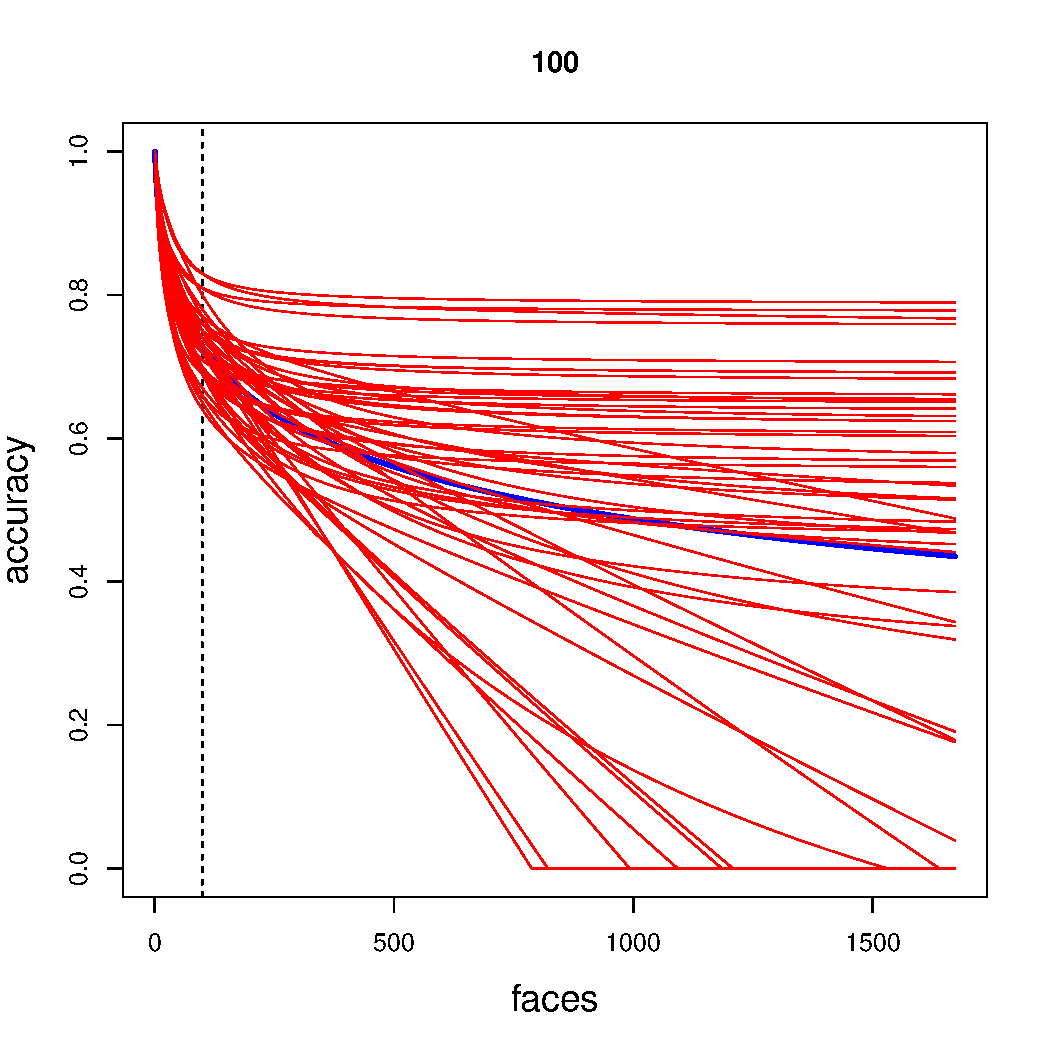
\includegraphics[scale = 0.4]{sub_100.pdf} &
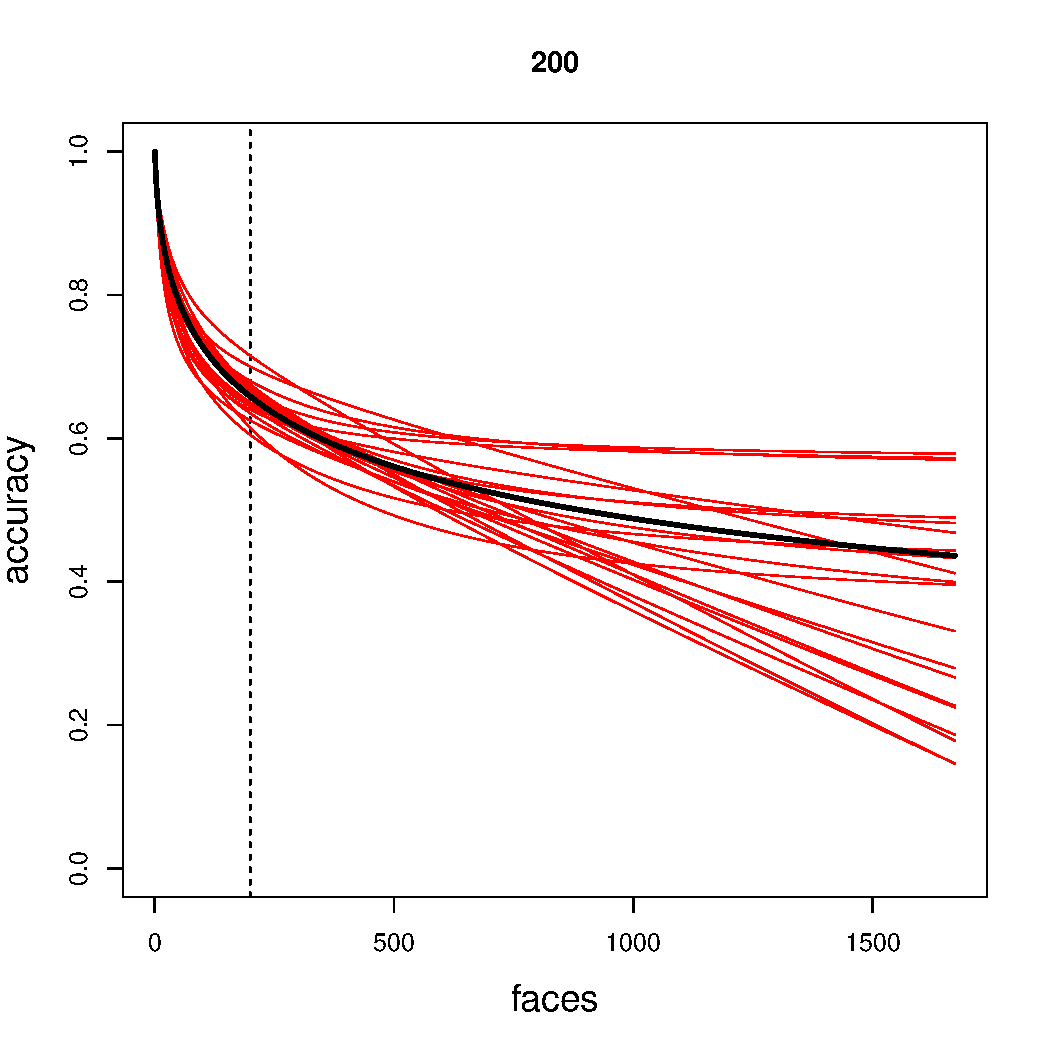
\includegraphics[scale = 0.4]{sub_200.pdf} \\
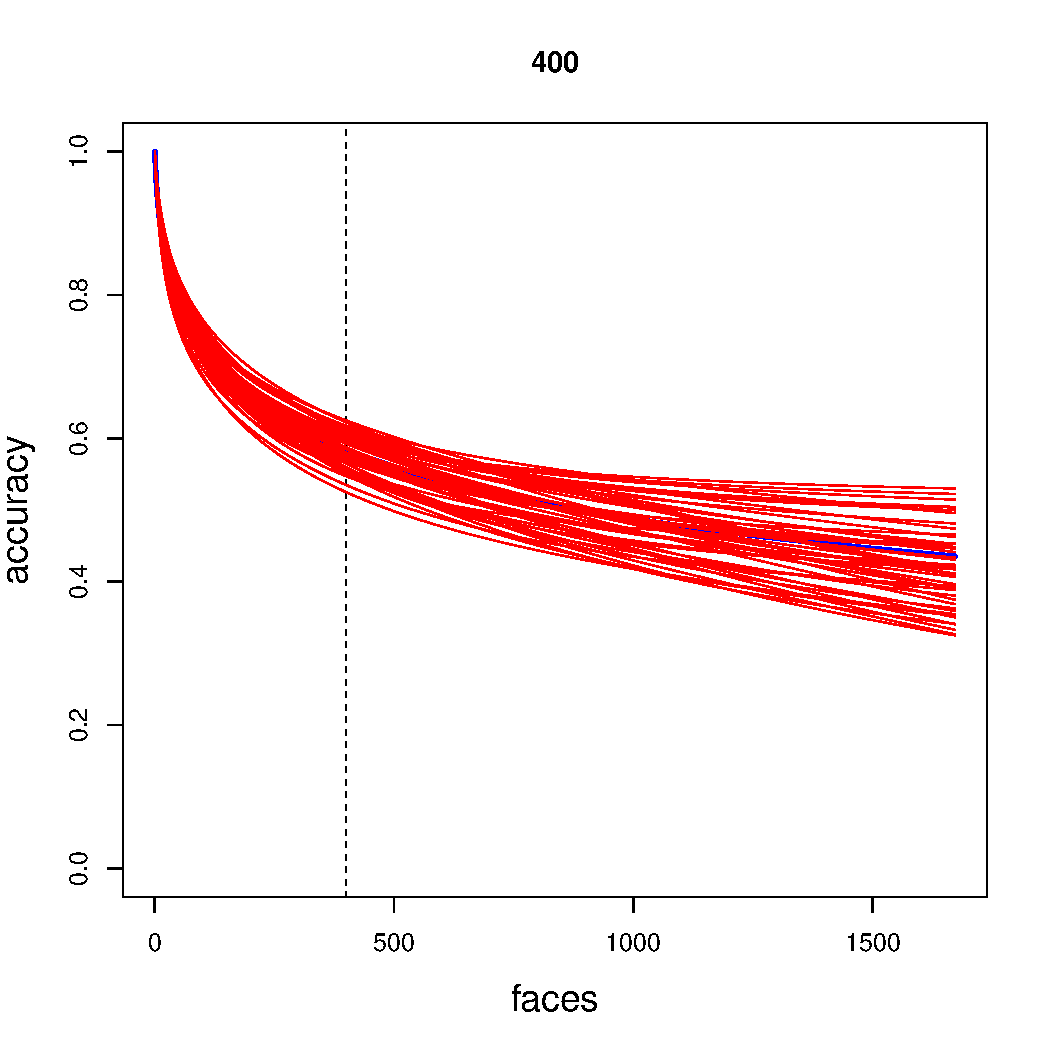
\includegraphics[scale = 0.4]{sub_400.pdf} &
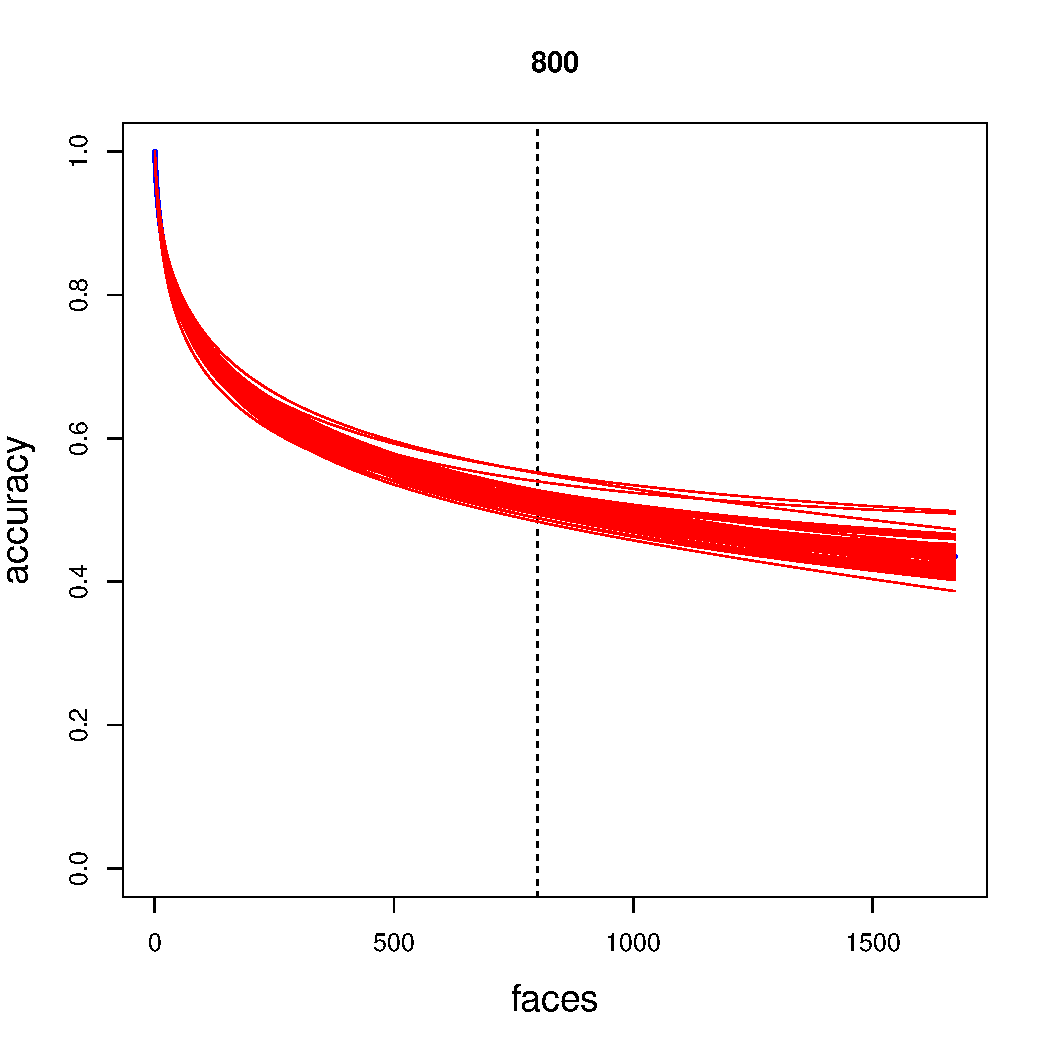
\includegraphics[scale = 0.4]{sub_800.pdf} 
\end{tabular}
\caption{Estimated average accuracy using subsampled datasets of size
  $k$, compared to the ground truth (average $k$-class test accuracy
  using all 1672 classes).}
\label{fig:lfw_extrapolation2}
\end{figure}

\subsection{Telugu OCR example}

While the previous example was a perfect fit to the assumptions of the
framework, we also want to see how well the method works when some of
the assumptions may be violated.  Towards this end we apply performance
extrapolation in an optical character recognition example
(\cite{achanta2015telugu}) for predicting the accuracy on 400 classes
of Telugu characters from a subsample of size $K = 20$.  We consider
the use of five different classifiers: Naive Bayes, logistic
regression, SVM, $\epsilon$-nearest neighbors\footnote{$k$-nearest
  neighbors with $k = \epsilon n$ for fixed $\epsilon > 0$}, and a
deep convolutional neural network\footnote{The network architecture is
  as follows: {\tt
    48x48-4C3-MP2-6C3-8C3-MP2-32C3-50C3-MP2-200C3-SM.}}.  Of the five
classifiers, only Naive Bayes satisfies the marginal classifier
assumption.  Again, we compare the result of our model to the ground
truth obtained by using the full dataset.

\begin{table}
\centering
\begin{tabular}{|c||c|c|c|}\hline
Classifier      & Test $\text{acc}^{(20)}$ & Test $\text{acc}^{(400)}$ & $\hat{AGA}_{400}$ \\ \hline
Naive Bayes     & 0.951                   & 0.601                   & 0.858     \\ \hline
Logistic        & 0.922                   & 0.711                   & 0.812     \\ \hline
SVM             & 0.860                   & 0.545                   & 0.687     \\ \hline
$\epsilon$-NN   & 0.951                   & 0.591                   & 0.410     \\ \hline
Deep neural net & 0.995                   & 0.986                   & 0.907     \\ \hline
\end{tabular}
\caption{Performance extrapolation: predicting the accuracy on 400 classes using data from 20 classes on a Telugu character dataset.
$\epsilon = 0.002$ for $\epsilon$-nearest neighbors.}
\label{tab:telugu}
\end{table}

The results are displayed in Table \ref{tab:telugu}.  To our surprise,
the worst absolute difference between ground truth and estimated
average accuracy was in the case of Naive bayes $(|\delta| = 0.257)$
which satisfies the marginal property.  All other classifiers had
absolute errors less than 0.2.  It is also interesting to note that,
even though Naive Bayes and $\epsilon$-nearest neighbors have the same
test accuracy on the subset, that the predicted accuracy on 400
differs greatly between then (0.858 vs 0.400).  Furthermore, the
difference is in the right direction: Naive Bayes is predicted to work
better on 400 classes than $\epsilon$-nearest neighbors, which appears
to be the case based on the 400-class test accuracy.

While further work is still needed to better understand the
performance of the proposed performance extrapolation method, both for
marginal classifiers (which satisfy the theoretical assumptions) and
non-marginal classifiers (which do not), the results obtained in these
two examples are encouraging in that sense that useful predictions
were obtained both for marginal and non-marginal classifiers.


\printbibliography[heading=bibintoc]

\end{document}






















